\documentclass[
  12pt,
  oneside,
  a4paper
  ]{report}
%%%%%%%%%%%%
% Packages %
%%%%%%%%%%%%
\usepackage[utf8]{inputenc}
\usepackage[
  rmargin=2.5cm,
  lmargin=3.5cm,
  tmargin=2.5cm,
  bmargin=2.5cm
  ]{geometry}
% \usepackage{showframe}
\usepackage{thesis}

%%%%%%%%%%%%%%%
% Definitions %
%%%%%%%%%%%%%%%
\definecolor{lacivert}{rgb}{0.0, 0.00, 0.52}

%%%%%%%%%%%%%%%%%%%%
% Defined Commands %
%%%%%%%%%%%%%%%%%%%%
% \DeclarePairedDelimiter{\abs}{\lvert}{\rvert}
% \DeclarePairedDelimiter{\norm}{\lVert}{\rVert}
\DeclarePairedDelimiter{\card}{\lvert}{\rvert}

\DeclareMathOperator*{\argmax}{arg\,max}
\DeclareMathOperator*{\argmin}{arg\,min}
\DeclareMathSymbol{\omicron}{\mathord}{letters}{"6F}

\newcommand{\rangedots}{\mathinner {\ldotp \ldotp}}
\newcommand{\concat}{\; \middle| \;}
\newcommand\orient[1]{\mathop{\rm{orient}}(#1)}
\newcommand\rbrkt[1]{\left(#1\right)}
\newcommand\sqbrkt[1]{\left[#1\right]}
\newcommand\cbrkt[1]{\left\{#1\right\}}
\newcommand\abrkt[1]{\langle#1\rangle}
\newcommand\set[1]{\left\{ \, #1 \, \right\}}
\newcommand\Set[2]{\left\{ \, #1 \; \colon \; #2 \, \right\}}
\renewcommand{\d}[1]{\ensuremath{\operatorname{d}\!{#1}}}

\newcommand{\TODO}[1]{\textcolor{red}{[\texttt{TODO:} #1]}}
\newcommand{\NOTE}[1]{\textcolor{lacivert}{[\texttt{NOTE:} #1]}}
\newcommand{\CITE}{\textcolor{purple}{[\texttt{CITE}]}}

%%%%%%%%%%%%
% Settings %
%%%%%%%%%%%%
\bibliographystyle{unsrtnat}

%%%%%%%%%%%%%%%%%%%%%%%%
% Thesis Main Document %
%%%%%%%%%%%%%%%%%%%%%%%%
\begin{document}

\title{}
\author{Ali Osman Berk Şapcı}
\maketitle

\tableofcontents
\listoffigures
\listoftables

\begin{abstract}
	A \textit{Bastı} (English: \textit{Basty}, Azerbaijani Turkish: \textit{Basdı}, Anatolian Turkish: \textit{Basdırık}) is an evil spirit in Turkic mythology which rides on people's chests while they sleep, bringing on  nightmares.
	Bastı sits astride a sleeper's chest and becomes heavier until the crushing weight awakens the terrified and breathless dreamer.
	The victim awakes, unable to move under the Bastıs weight.
	It may also include lucid dreams.
	% There are different types of Bastı in Anatolia: Al-Bastı, Kara-Bastı, Kul-Bastı, Sarı-Bastı.
\end{abstract}

\setlength{\parindent}{0pt}
\chapter{Introduction}\label{chapter:introduction}
Sleep is an essential behavioral program conserved across the animal kingdom, in diverse species ranging from jellyfish to humans, whose function
remains unknown \citep{campbell_animal_1984, nath_jellyfish_2017}.
In mammals, sleep consists of multiple stages marked by physiological changes, including reductions in muscle tone and distinct electrophysiological activity patterns in the brain \citep{corner_sleep_1977, sauer_dynamics_2003}
In invertebrates, sleep has largely been studied as a unitary process and identified by bouts of consolidated immobility.
Thus, careful characterization of underlying changes in behavior and physiology is needed for understanding the functional role of the sleep, and characterizing distinct sleep stages in powerful genetic model systems such as \textit{Drosophila Melanogaster}.


\NOTE{
	\begin{itemize}
		\item Computational {Neuroethology}: {A} {Call} to {Action}: \citep{datta_computational_2019}
		\item Quantifying behavior to understand the brain: \citep{pereira_quantifying_2020}
		\item Toward a {Science} of {Computational} {Ethology}: \citep{anderson_toward_2014}
	\end{itemize}
}
\NOTE{
	\begin{itemize}
		\item Mapping {Sub}-{Second} {Structure} in {Mouse} {Behavior}
		\item 	{DeepLabCut}: markerless pose estimation of user-defined body parts with deep learning: \citep{mathis_deeplabcut_2018}
		\item Fast animal pose estimation using deep neural networks: \citep{pereira_fast_2019}
		\item {SLEAP}: {A} deep learning system for multi-animal pose tracking: \citep{pereira_sleap_2022}
	\end{itemize}
}

\NOTE{
	\begin{itemize}
		\item A deep sleep stage in {Drosophila} with a functional role in waste clearance: \citep{van_alphen_deep_2021}
		\item Most sleep does not serve a vital function: {Evidence} from {Drosophila} melanogaster: \citep{geissmann_most_2019}
		\item Automated analysis of long-term grooming behavior in {Drosophila} using a k-nearest neighbors classifier: \citep{qiao_automated_2018}
		\item Mapping the stereotyped behaviour of freely moving fruit flies: \citep{berman_mapping_2014}
		\item Systematic exploration of unsupervised methods for mapping behavior: \citep{todd_systematic_2017}
	\end{itemize}
}
\NOTE{
	\begin{itemize}
		\item Predictability and hierarchy in \textit{{Drosophila}} behavior: \citep{berman_predictability_2016}
		\item The manifold structure of limb coordination in walking {Drosophila}: \citep{deangelis_manifold_2019}
		\item The 103,200-arm acceleration dataset in the {UK} {Biobank} revealed a landscape of human sleep phenotypes: \citep{katori_103200-arm_2022}
	\end{itemize}
}
\NOTE{
	\begin{itemize}
		\item A dictionary of behavioral motifs reveals clusters of genes affecting {Caenorhabditis} elegans locomotion: \citep{brown_dictionary_2013}
		\item Deconstructing {Hunting} {Behavior} {Reveals} a {Tightly} {Coupled} {Stimulus}-{Response} {Loop}: \citep{mearns_deconstructing_2020}
		\item Continuous {Whole}-{Body} {3D} {Kinematic} {Recordings} across the {Rodent} {Behavioral} {Repertoire} - {SI}: \citep{marshall_continuous_2021}
		\item Mapping {Sub}-{Second} {Structure} in {Mouse} {Behavior}: \citep{wiltschko_mapping_2015}
		\item The {Mouse} {Action} {Recognition} {System} ({MARS}) software pipeline for automated analysis of social behaviors in mice: \citep{segalin_mouse_2021}
		\item Neural control of affiliative touch in prosocial interaction: \citep{wu_neural_2021}
		\item Partitioning variability in animal behavioral videos using semi-supervised variational autoencoders: \citep{whiteway_partitioning_2021}
		\item Structure of the {Zebrafish} {Locomotor} {Repertoire} {Revealed} with {Unsupervised} {Behavioral} {Clustering}: \citep{marques_structure_2018}
	\end{itemize}
}

\NOTE{
	\begin{itemize}
		\item {DeepEthogram}, a machine learning pipeline for supervised behavior classification from raw pixels: \citep{bohnslav_deepethogram_2021}
		\item B-{SOiD}, an open-source unsupervised algorithm for identification and fast prediction of behaviors: \citep{hsu_b-soid_2021}
		\item Ethoscopes: {An} open platform for high-throughput ethomics: \citep{geissmann_ethoscopes_2017}
		\item {JAABA}: interactive machine learning for automatic annotation of animal behavior: \citep{kabra_jaaba_2013}
		\item Simple {Behavioral} {Analysis} ({SimBA}) – an open source toolkit for computer classification of complex social behaviors in experimental animals: \citep{nilsson_simple_2020}
	\end{itemize}
}

\chapter{Experiments and Data Collection}\label{chapter:expt-data-collection}
In this section, we describe how the sleep experiments are conducted and fly video recordings data were collected.

\section{Sleep Experiments and Video Recordings}

\textit{The experimental data was collected by Dr. Mehmet Fatih Keles at Johns Hopkins University.}

A custom imaging setup was used to perform high-resolution characterization of sleep-related behaviors in flies. This set up includes a custom 3D printed chamber (7.2X4.3X2.4 mm [WxHxL]) that is placed in front of an IR sensitive (Flir) 30 FPScamera with telecentric lens (Edmund Optics).

\begin{figure}[ht!]
	\centering
	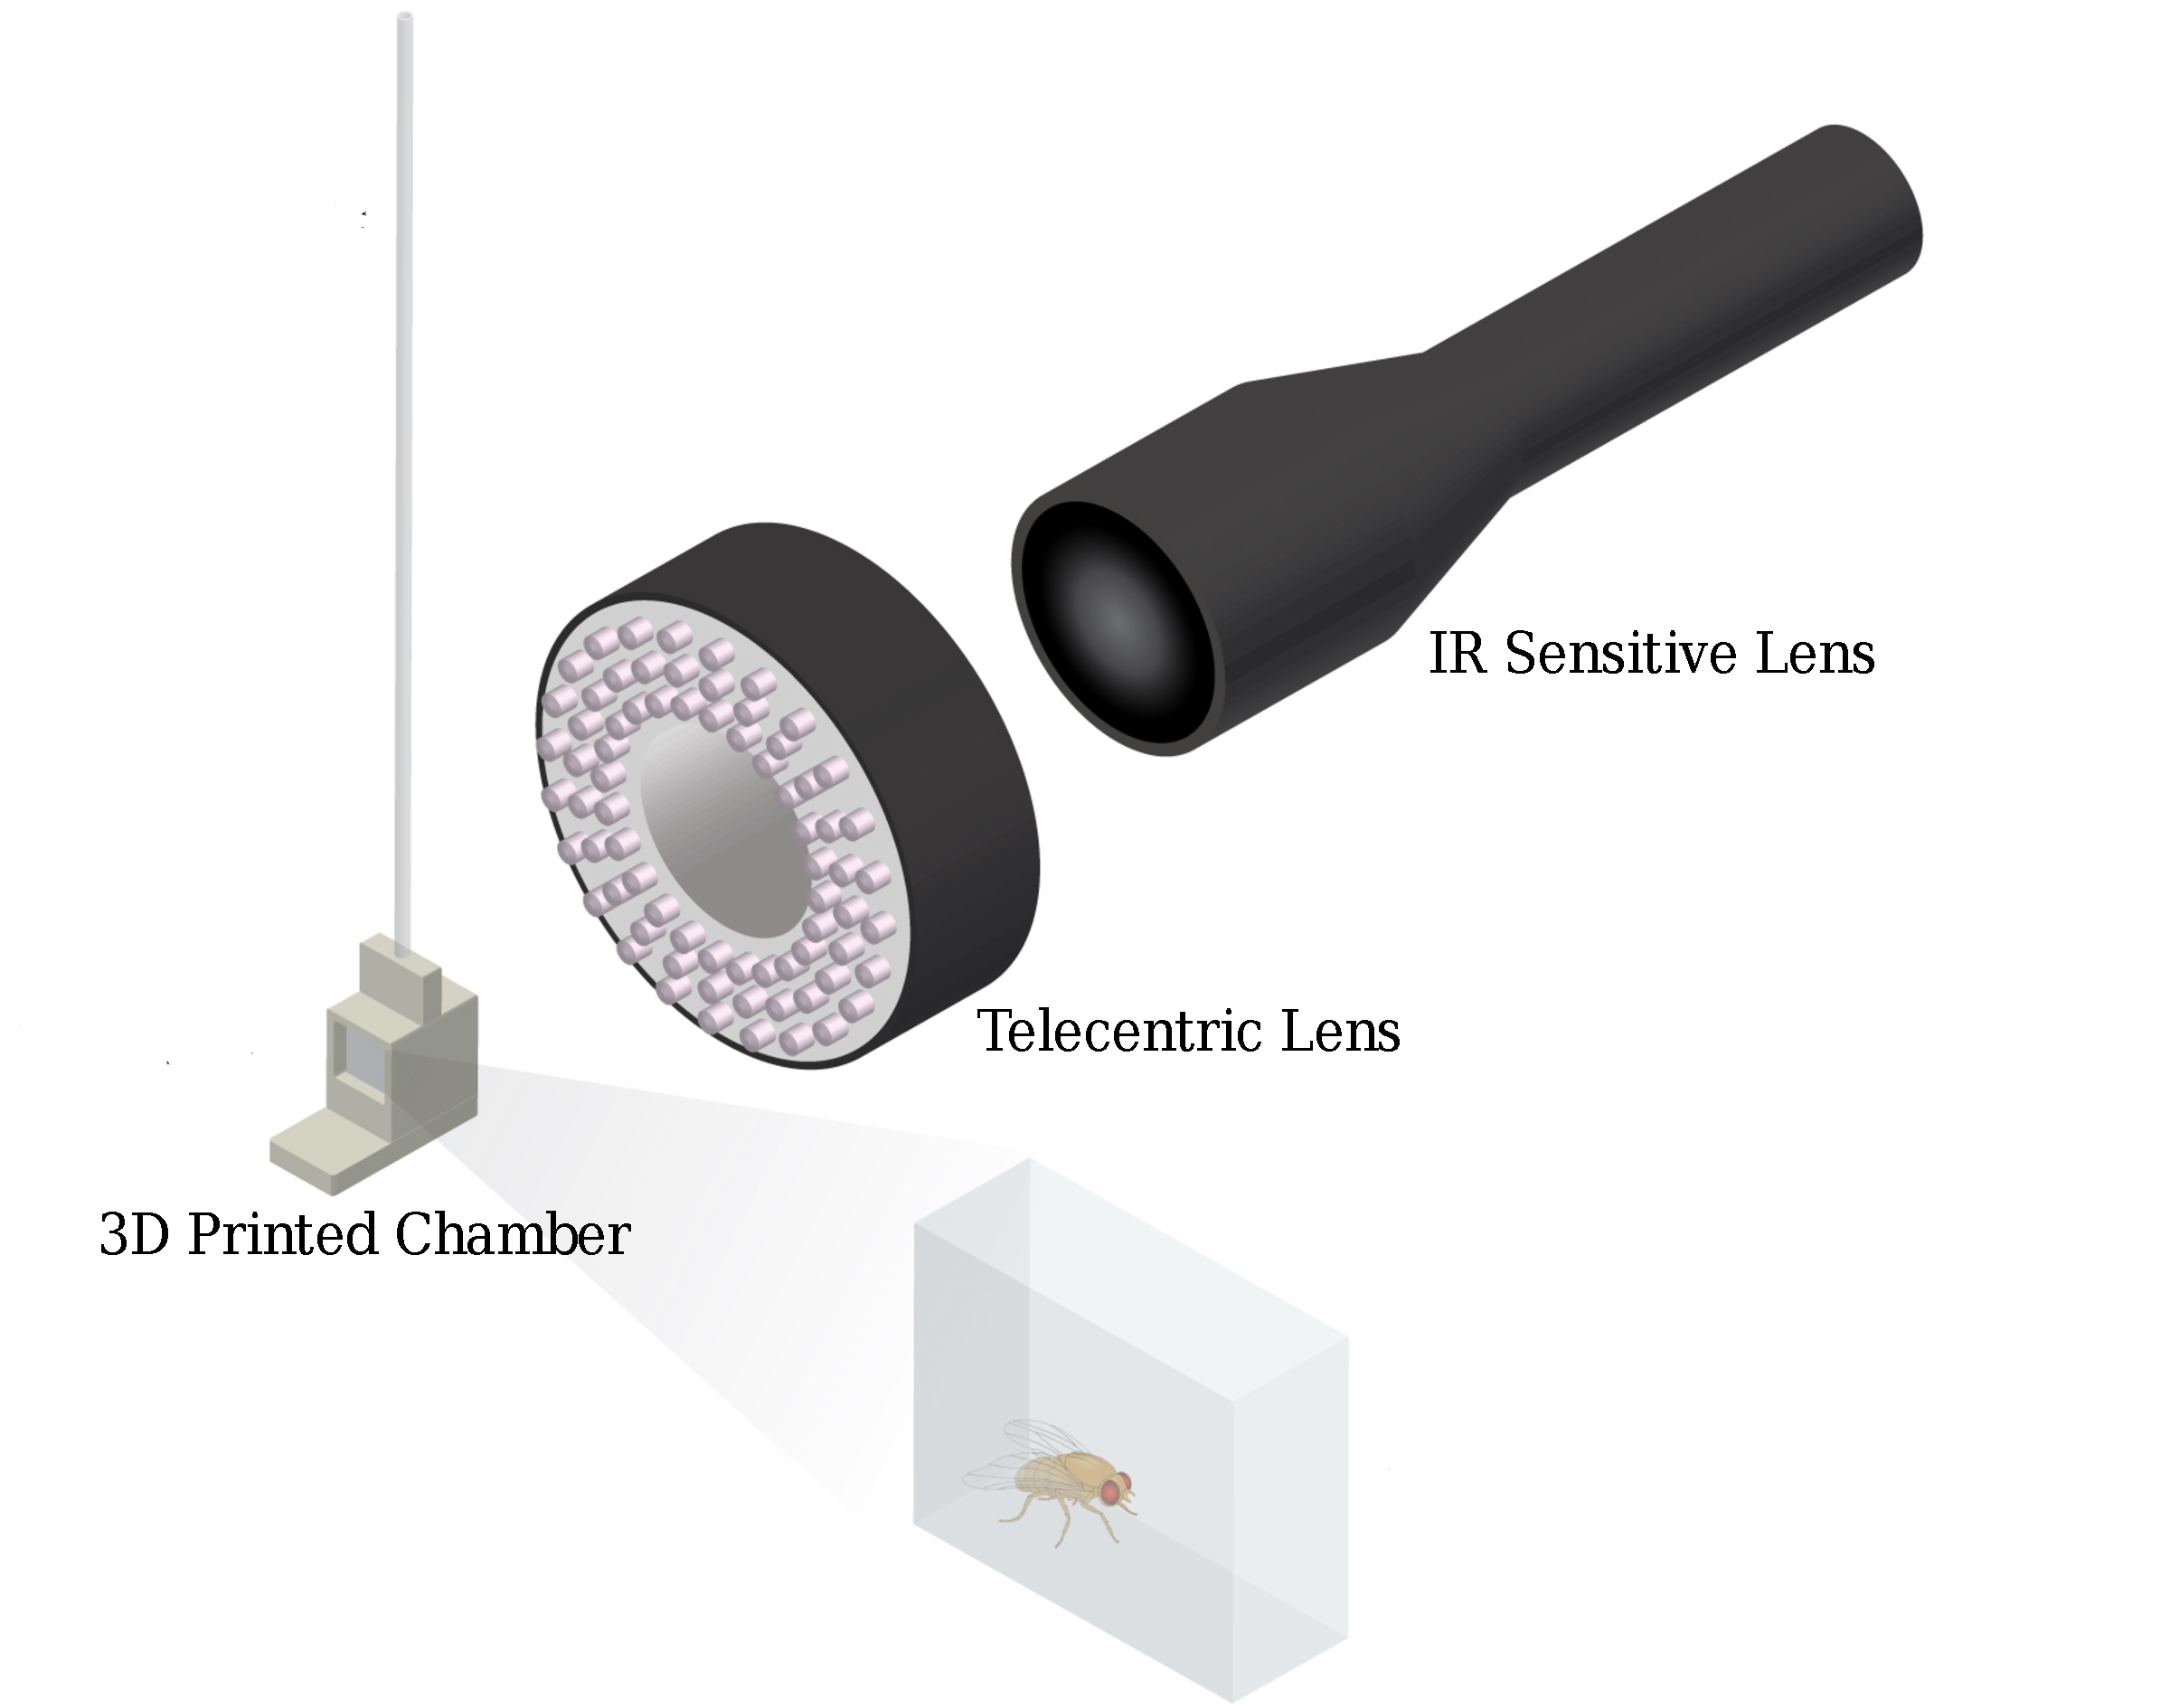
\includegraphics[width=0.75\linewidth]{figures/ExperimentalSetup.pdf}
	\caption[An illustration of the experimental setup which is used to perform high-resolution imaging of experiments.]{An illustration of the experimental setup which is used to perform high-resolution imaging of experiments.}
\end{figure}

Flies recorded from ZT10-ZT2 (16 hours) total.
Each chamber has a food port (1.5mm diameter) that allows access to liquid food (2.5\% yeast, 2.5\% sugar).
Recording setup is in light tight box and humidity control (60\%) is achieved via humidifier plugged into a humidity control switch. Experimental flies are loaded to individual chambers at ZT8-ZT9 via mouth pipette or a small vacuum pump.
Individual chambers are sealed with a 7x7 mm acrylic windows.
Windows are coated with SigmaCote to prevent flies from ventral or dorsal postural positions. 5-7 day old female and male flies are used in the experiments.

\section{Pose Estimation and Tracking}
A recently developed deep neural network based software, DeepLabCut was used to achieve markerless pose estimation.
Over 20 body parts are first labeled in 1654 images from 28 animals (16 female, 12 male) to train the model with a 95/5 train/test split.
We used a ResNet-50 based neural network with a batch size of 4 and 200k training iterations.
Rest of the settings were kept default.
The resulting network has a test error of 3.67 pixels.

\begin{figure}[ht!]
	\centering
	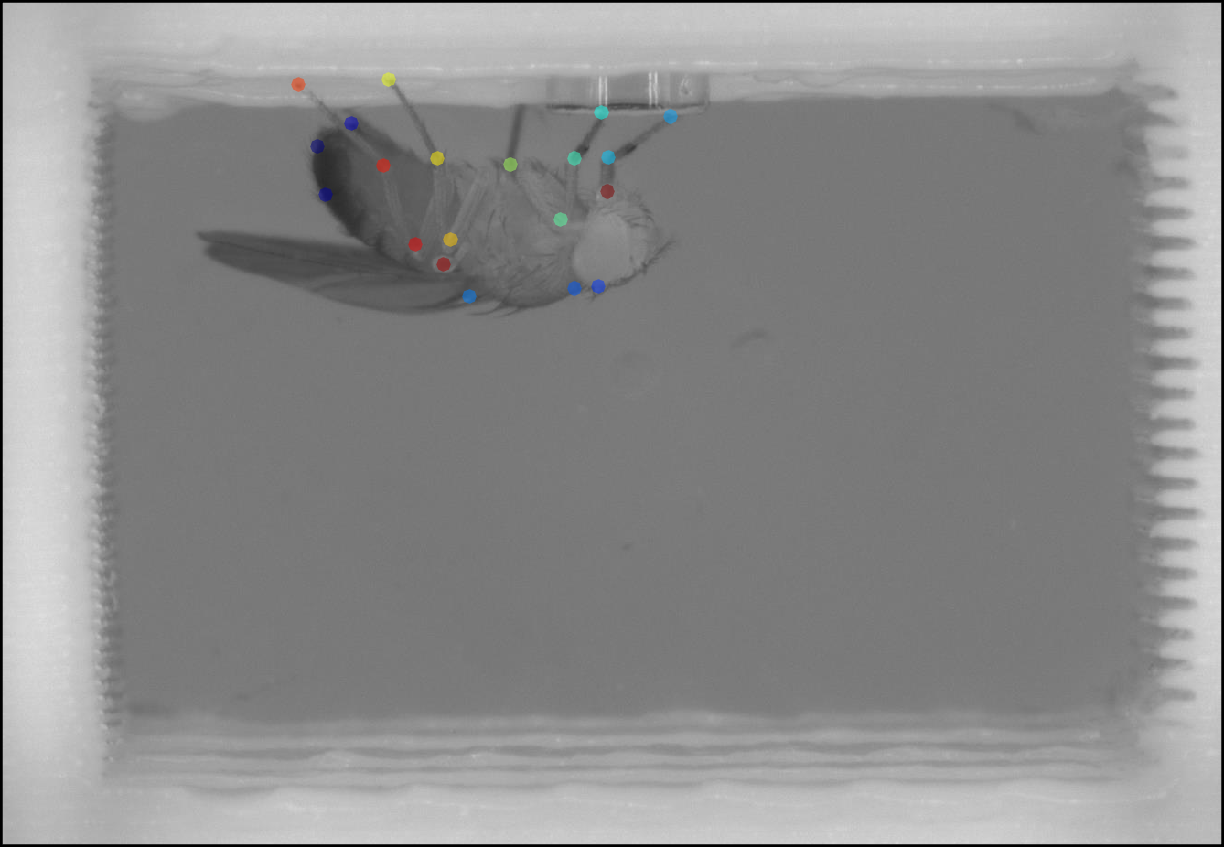
\includegraphics[width=0.75\linewidth]{figures/FlyTrackedBodyParts.png}
	\caption[An example frame of the fruit fly placed in 3D printed chamber.] {An example video recording frame of the fruit fly placed in 3D printed chamber. Colorful markers indicates the tracked body parts.}
\end{figure}

\section{Behavior Annotations}

3 human annotators labeled 5 different behaviors (feeding, grooming, moving, haltere switch, proboscis pumping) across 11 videos (14 hours and 16 hours each, respectively for 7 wild type sleep experiments and 4 sleep deprivation experiments).
A single experiment is annotated by all 3 annotators to check rigor and overlap among annotators. We only used the annotations of a fly on when  annotators agreed at least on the 90\% of the labels.

\begin{figure}[ht!]
	\centering
	\begin{subfigure}[ht!]{0.95\linewidth}
		\centering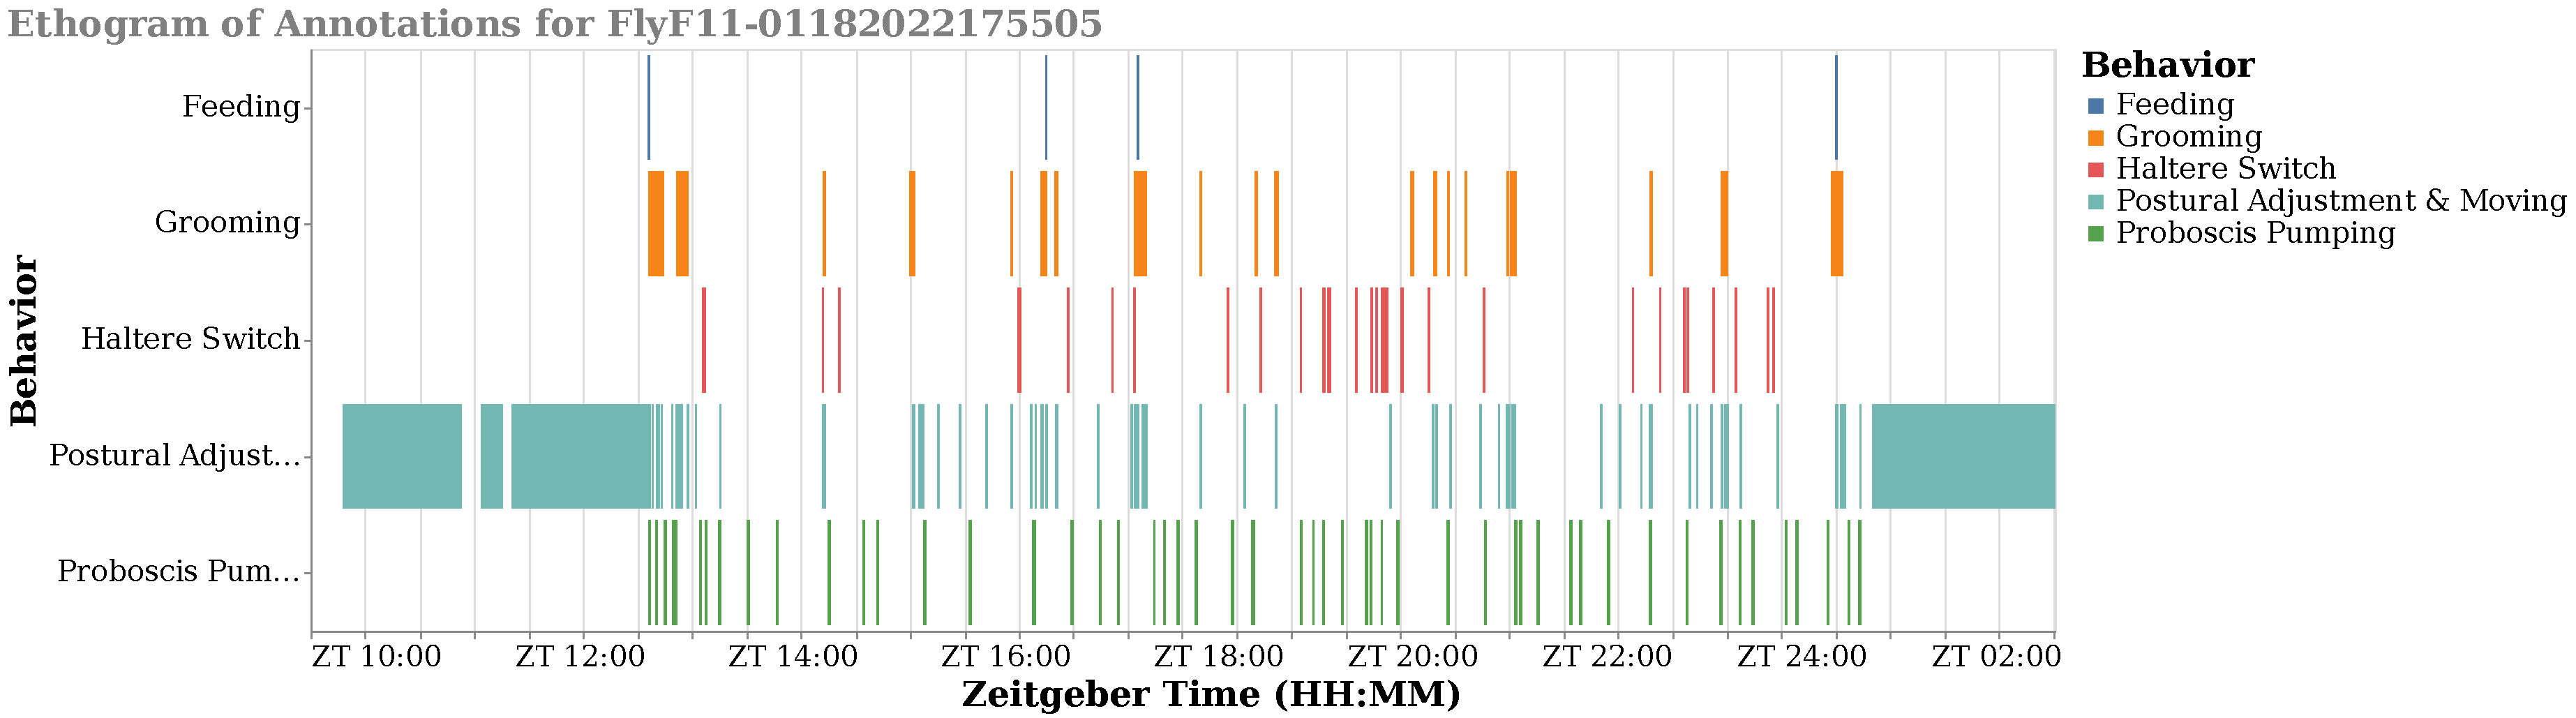
\includegraphics[width=\linewidth]{figures/FlyF11-01182022175505_annotation_ethogram.pdf}
		\caption{Wild type.}
	\end{subfigure}%

	\centering
	\begin{subfigure}[ht!]{0.95\linewidth}
		\centering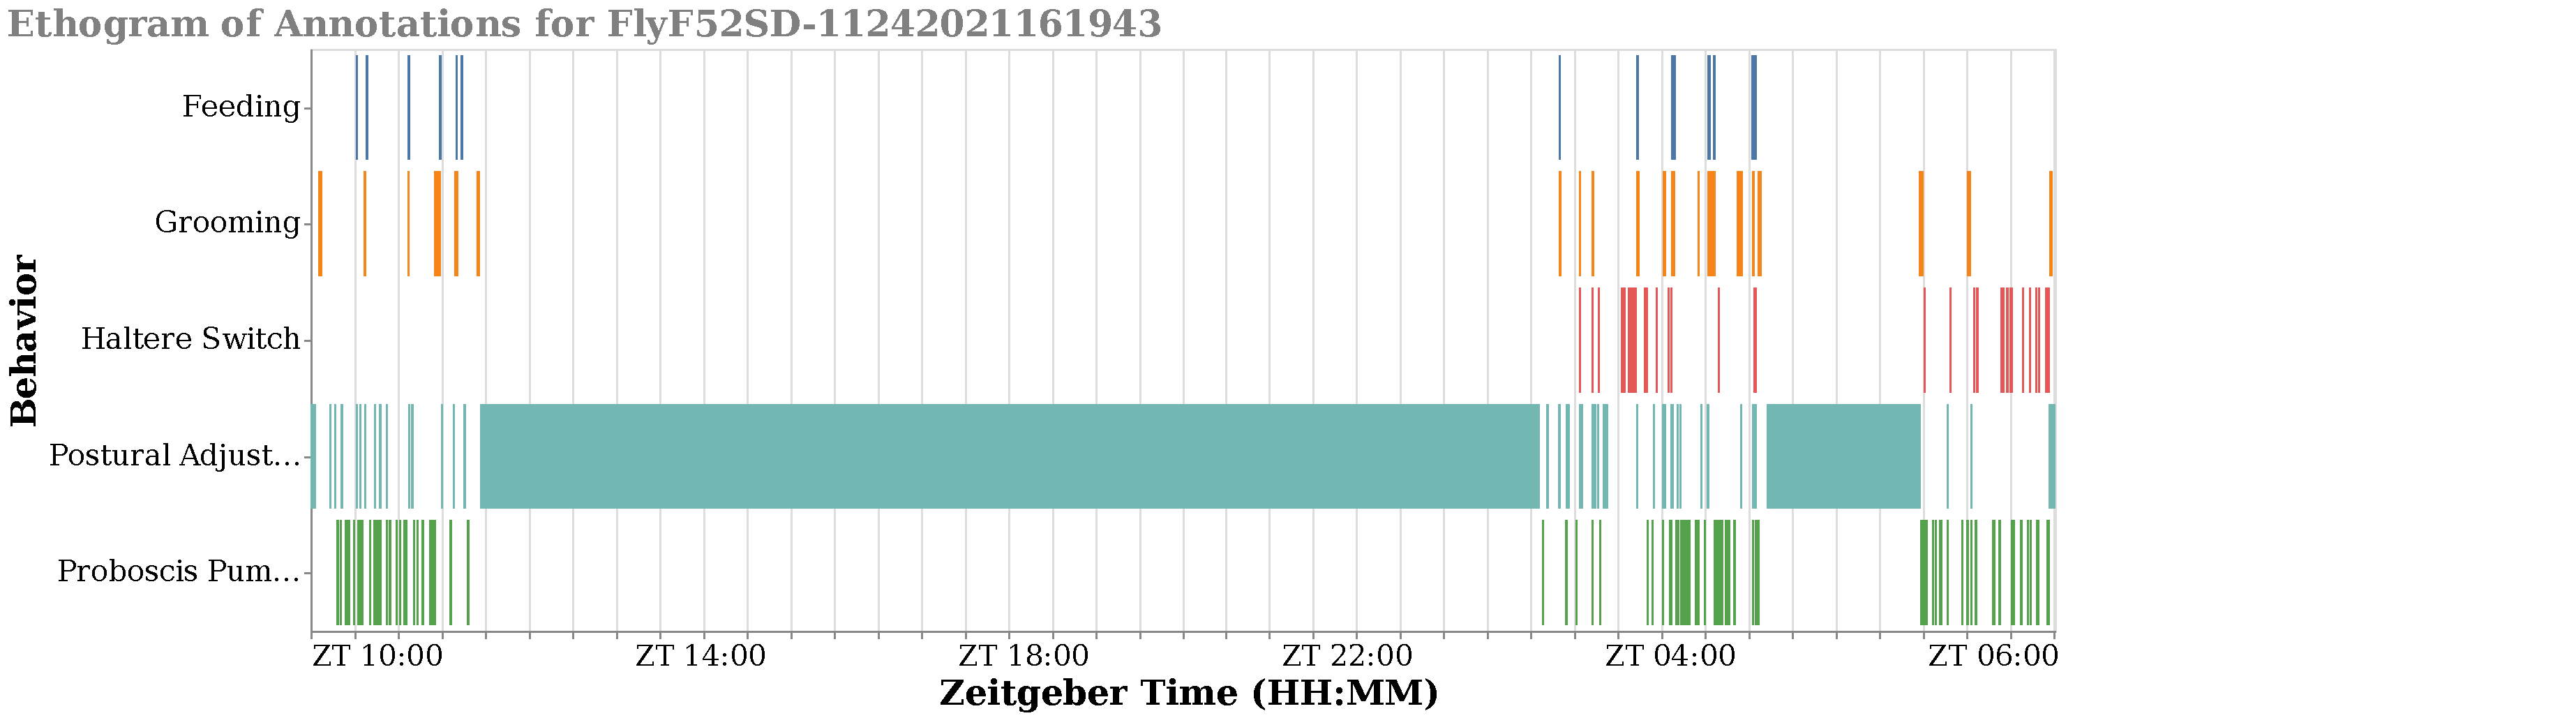
\includegraphics[width=\linewidth]{figures/FlyF52SD-11242021161943_annotation_ethogram.pdf}
		\caption{Sleep deprived.}
	\end{subfigure}%
	\caption[Two example ethograms of annotated behaviors observed during the sleep experiments.]{Two example ethograms of annotated behaviors observed during the sleep experiments. Dark period starts at ZT 12, and ends at ZT 0.}
\end{figure}

\chapter{Feature Extraction}
For a single experiment data, feature extraction consists of four consecutive steps, where the input in a stage is the output of the previous one.
The input of the first step is the raw output signal of the tracking and pose estimation model, in our case, the output of DeepLabCut.
The feature extraction steps are as follows:

\begin{enumerate}
	\item Constructing pose values and preprocessing (filtering and imputation).
	\item Computing spatio-temporal features, such as distances between body parts, velocity, angular velocity from body part positions.
	\item Extending spatio-temporal features to multiple time-scales using wavelet transformation and sliding window statistics.
	\item Computing high-dimensional behavioral representations with normalization.
\end{enumerate}

Matrices $\mathbf{X} \in \mathbb{R}^{T \times N}$ and $\mathbf{Y} \in \mathbb{R}^{T \times N}$ denotes a multivariate time series collected for $N$ tracked body part of the fly on $T$ time stamps by a pose estimation model, respectively for $x$ and $y$ cartesian components of two-dimensional video recordings. This multivariate time series matrices $\mathbf{X}$ and $\mathbf{Y}$ are the raw input data to the first step of the feature extraction.
Note that $N$ must be the same among all experiments conducted with different fruit flies, but $T$ might differ.
Each column of the $\mathbf{X}=[\mathbf{x}_1, \cdots, \mathbf{x}_N]^\top$ and $\mathbf{Y}=[\mathbf{y}_1, \cdots, \mathbf{y}_N]^\top$ can be written respectively as follows;

\begin{align*}
	\mathbf{y}_i & = (y_{i,1}, y_{i,2}, \dots, y_{i,t-1}, y_{i,t}, y_{i,t}, \dots, y_{i,T}), \\
	\mathbf{x}_i & = (x_{i,1}, x_{i,2}, \dots, x_{i,t-1}, x_{i,t}, x_{i,t}, \dots, x_{i,T}).
\end{align*}

Here $i$ denotes the index of the body part, e.g. leg tip or proboscis.


In addition to $\mathbf{X}$ and $\mathbf{Y}$, many tracking and pose estimation models report prediction scores for each tracked body part at each time step.
$L \in \mathbb{R}^{N \times T}$ denotes the time series of prediction scores, each column of the $L=[l_1, \cdots, l_N]^\top$ can be written as follows;

\begin{equation*}
	\mathbf{l}_i = (l_{i,1}, l_{i,2}, \dots, l_{i,t-1}, l_{i,t}, l_{i,t}, \dots, l_{i,T}).
\end{equation*}

The prediction score drops drastically when the body part is not visible. Thus, $L$ provides valuable information about the occluded body parts. In the Section~\ref{section:dealing-with-occluded-body-parts}, how $L$ is incorporated into construction of pose values is described in detail.

\section{Construction of Pose Values and Preprocessing}
The goal of this sub-stage is primarily preprocessing, which involves filtering and imputation certain frames.
But in addition to this, there are a couple of optional procedures that can be beneficial for our task of learning stereotypical behaviors.
These additional procedures deal with occluded body parts of the fly, alignment of the fly orientations and defining new points of interest.

\subsection{Dealing with Occluded Body Parts}\label{section:dealing-with-occluded-body-parts}
As mentioned in the Section~\ref{section:challanges}, the two-dimensional video recordings introduces a number of important challenges, and one of them is the occluded body part challenge.
There are many types of occlusions which can be informally described as follows.
One examples is short occlusions resulting from postural changes.
Imputation of the time series $\mathbf{X}$ and $\mathbf{Y}$ for these short occlusions is relatively easy since the number of missing data points are  few.
However, this is not the case for long occlusions which usually occur when the fly is dormant for a long period of time.
Especially for the body parts which have left and right counterparts, it is common that the orientation of the fly results in one of the counterparts being occluded in long dormant epochs.
We follow multiple approaches to handle different type occlusions; namely imputation and elimination of corresponding data-points.
Before describing those approaches we define a criterion for being occluded.

\subsubsection{Computing Oriented Pose Values to Handle Body Parts with Left \& Right Counterparts}
If the fly oriented perpendicular to the camera perspective as in Figure~\ref{figure:perpendicular-orientation}, then one of the left and right body parts is often occluded.
In other orientations (e.g. Figure~\ref{figure:parallel-orientation} and Figure~\ref{figure:oblique-orientation}),  both of them or none of them might be occluded as well.
However, in the conducted experiments, flies usually choose to stay dormant perpendicular to the camera perspective in long dormant epochs, as mentioned in Chapter~\ref{chapter:expt-data-collection}.
In such cases, one can only use one of the left and right counterparts to construct pose values.
Therefore, this optional step is included in the behavioral mapping pipeline to reduce pose values of body parts with left and right counterparts to a single value.

We use prediction scores to determine which body part should be used to construct pose value.
Let $i$ and $j$ be a pair of body parts which are left and right counterparts of each other, e.g. left haltere and right haltere.
Then one can use the $\mathbf{l}_i$ and $\mathbf{l}_j$ to predict if one of them is occluded at a particular time step $t$.
Let $\orient{\mathbf{x}_i, \mathbf{x}_j}$ ($\orient{\mathbf{y}_i, \mathbf{y}_j}$) be a new pose vector which will be computed based on $\mathbf{x}_i$ and $\mathbf{x}_j$ ($\mathbf{y}_i$ and $\mathbf{y}_j$), e.g. an oriented haltere pose value from left haltere and right haltere.
The following conditional produces are proposed to compute oriented pose values from left and right pose values by deciding the orientation of the fly for that counterpart; they can be used separately or together.
\begin{itemize}
	\item If $l_{i,t} - l_{j,t} \geq  \epsilon$ then without loss of generality $\orient{x_{i,t}, x_{j,t}}=x_{i,t}$ and $\orient{y_{i,t}, y_{j,t}}=y_{i,t}$ for a threshold $\epsilon$, typically $\epsilon > 0.5$.
	\item If $\card{\Set{t^{\prime}}{l_{i,t^{\prime}} > l_{j,t^{\prime}}, t^{\prime} \in [t-w \rangedots t+w]}} > w$, then without loss of generality $\orient{x_{i,t}, x_{j,t}}=x_{i,t}$ and $\orient{y_{i,t}, y_{j,t}}=y_{i,t}$ for a window size $2w+1$.
	\item If $l_{i,t} > l_{j,t}$ and $\abs{t-t^i} < \abs{t-t^j}$ where $t^i=\argmin_{t^i} \abs{t-t^i}$, $t^i \in \Set{t^{\prime}}{l_{i,t^{\prime}} - l_{j,t^{\prime}} > \epsilon}$ and $t^j=\argmin_{t^j} \abs{t-t^j}$, $t^j \in \Set{t^{\prime}}{l_{j,t^{\prime}} - l_{i,t^{\prime}} > \epsilon}$ for some threshold $\epsilon$ then without loss of generality $\orient{x_{i,t}, x_{j,t}}=x_{i,t}$ and $\orient{y_{i,t}, y_{j,t}}=y_{i,t}$.
	\item If simply $l_{i,t} > l_{j,t}$ (i.e. hard threshold) then without loss of generality $\orient{x_{i,t}, x_{j,t}}=x_{i,t}$ and $\orient{y_{i,t}, y_{j,t}}=y_{i,t}$.
\end{itemize}
Except applying a hard threshold, all other conditions may leave some of the time points with undecided orientations.
If the number of such time points is acceptable, then applying hard threshold for those time points is convenient and handy.

After applying above procedures for one right and left counterpart pair $i, j$, we can define
\begin{align*}
	\mathbf{X}^{\ast} & = \rbrkt{[(\mathbf{x}_p)_{p \notin \cup\mathcal{O}}] \mid [\left(\orient{\mathbf{x}_i, \mathbf{x}_j}\right)_{\set{i,j} \in \mathcal{O}}]}^\top,      \\
	\mathbf{Y}^{\ast} & = \rbrkt{[(\mathbf{y}_p)_{p \notin \cup\mathcal{O}}] \mid [\left(\orient{\mathbf{y}_i, \mathbf{y}_j}\right)_{\set{i,j} \in \cup \mathcal{O}}]}^\top. \\
\end{align*}
\begin{align*}
	\mathbf{X}^{\ast} & =\rbrkt{ (x_{p,t})_{t \in \set{1, \cdots, T}, p \notin \cup \mathcal{O}} \mid [\left(\orient{\mathbf{x}_i, \mathbf{x}_j}\right)_{\set{i,j} \in \mathcal{O}}]}^\top,   \\
	\mathbf{Y}^{\ast} & = \rbrkt{(y_{p,t})_{t \in \set{1, \cdots, T}, p \notin \cup \mathcal{O}}  \mid  [\left(\orient{\mathbf{x}_i, \mathbf{x}_j}\right)_{\set{i,j} \in \mathcal{O}}]}^\top. \\
\end{align*}
where $\mathcal{O}$ is the set of index pairs of right and left counterparts and $\cup \mathcal{O}$ is the union of all such indexes.
Applying this procedure for each right and left counterparts results in computing $\mathbf{X}^{\ast}$ and $\mathbf{Y}^{\ast}$.
This oriented version of original data matrices can be used instead of $\mathbf{X}$ and $\mathbf{Y}$ in the rest of the pipeline, if desired.

\subsubsection{Detecting Occlusions Using Prediction Scores and Preternatural Tracking Predictions}

\subsection{Aligning Flies with Different Orientations}

\subsection{Preprocessing: Filtering and Imputation}

\section{Computation of Spatio-temporal Features from Pose Values}
Constructing pose values enables us to go one step further towards learning stereotypical behaviors.
Tracking of relevant body parts and constructing pose values is an essential step for quantifying behavior.
However, a set of coordinate values is sufficient to describe and represent complex spatio-temporal dynamics of animal behavior.
There are thousands of unique postures and behaviors are not exhibited by some static set of postures.
Instead, they are defined by expressive and meaningful spatio-temporal features such as distances, velocities, angles and angular velocities.
Therefor, one need to compute such features from the coordinate values of body parts in two dimensional space.

Second stage of the feature extraction is computation of spatio-temporal features from pose values. Two type of features are computed in this stage.
\begin{enumerate}
	\item \textbf{Snapshot features:} Spatio-temporal feature values computed at a snapshot of time.
	      \begin{itemize}
		      \item distances,
		      \item angles,
		      \item cartesian pose values (i.e. per body part features).
	      \end{itemize}
	\item \textbf{Gradient features:} Spatio-temporal feature values computed based how snap features change over time.
	      \begin{itemize}
		      \item change of distances,
		      \item change of angles (i.e. angular velocities),
		      \item change of cartesian pose values (i.e. body part velocities).
	      \end{itemize}
\end{enumerate}

The gradient of snapshot features computed using second order accurate central differences in the interior points. The returned gradient features has the same shape as the snapshot features.

\subsection{Distances Between body parts}
Given body part pair $\rbrkt{i,j}$, distances between them at a time step $t$ is computed as:
\begin{equation}
	d^{i,j}_t = \sqrt{(x_{i,t} - x_{j,t})^2 + (y_{i,t} - y_{j,t})^2}.
\end{equation}

The corresponding gradient feature, which is the change of distance between body part $i$ and $j$ is computed as follows using the second order gradient approximation:
\begin{equation}
	\dot{d}^{i,j}_t = \begin{cases} \frac{\abs{d^{i,j}_{t+1} - d^{i,j}_{t}}}{\Delta t} & \textnormal{if } $t=0$ \textnormal{ or } $t=T$, \\ \frac{\abs{d^{i,j}_{t+1} - d^{i,j}_{t-1}}}{2\Delta t} & \textnormal{otherwise}, \end{cases}
\end{equation}
where $\Delta t$ is the sampling period, which is equal to $\sfrac{1}{\textnormal{FPS}}$ seconds.

\subsection{Joint Angles Between body parts}
Given a triplet of body parts $\rbrkt{i,j,k}$, angle between $i$ and $k$ around $j$ is computed using the 2-argument arctangent function as below.
\begin{equation}
	w^{i,j,k}_t = \mathop{\rm{atan2}}\left(\det \begin{bmatrix} x_{i,t} - x_{j,t}, x_{k,t} - x_{j,t} \\ y_{i,t} - y_{j,t}, y_{k,t} - y_{j,t} \end{bmatrix}, \begin{bmatrix} x_{i,t} - x_{j,t} \\ y_{i,t} - y_{j,t} \end{bmatrix} \cdot \begin{bmatrix} x_{k,t} - x_{j,t}  \\ y_{k,t} - y_{j,t} \end{bmatrix}      \right) + \pi
\end{equation}

Then similar to distance gradient feature, angular velocity is approximated by:
\begin{equation}
	\dot{w}^{i,j,k}_t = \begin{cases} \frac{\abs{w^{i,j,k}_{t+1} - w^{i,j,k}_{t}}}{\Delta t} & \textnormal{if } $t=0$ \textnormal{ or } $t=T$, \\ \frac{\abs{w^{i,j,k}_{t+1} - w^{i,j,k}_{t-1}}}{2\Delta t} & \textnormal{otherwise}. \end{cases}
\end{equation}

\subsection{Cartesian Pose Values of body parts}
Cartesian pose values of a body part $i$ is straightforwardly given by the $x$ and $y$ coordinate values:
\begin{align}
	x^{i}_t & = x_{i,t}, \\
	y^{i}_t & = y_{i,t}.
\end{align}
Note that for a single body part two feature values is generated.

Corresponding gradient features, namely body part velocities along each cartesian component is computed as follows:
\begin{align}
	\dot{x}^{i}_t & = \begin{cases} \frac{x^{i}_{t+1} - x^{i}_{t}}{\Delta t} & \textnormal{if } $t=0$ \textnormal{ or } $t=T$, \\ \frac{x^{i}_{t+1} - x^{i}_{t-1}}{2\Delta t} & \textnormal{otherwise}, \end{cases} \\
	\dot{y}^{i}_t & = \begin{cases} \frac{y^{i}_{t+1} - y^{i}_{t}}{\Delta t} & \textnormal{if } $t=0$ \textnormal{ or } $t=T$, \\ \frac{y^{i}_{t+1} - y^{i}_{t-1}}{2\Delta t} & \textnormal{otherwise}. \end{cases}
\end{align}

\subsection{Constructing Spatio-temporal Feature Matrices}
Let $\mathcal{C}, \mathcal{D}$, and $\mathcal{A}$ denote set of body parts, body part pairs, body part triplets which defines snapshot features; respectively cartesian pose values, distances and angles.
Similarly, let $\mathcal{C}^{\prime}, \mathcal{D}^{\prime}$, and $\mathcal{A}^{\prime}$ denote sets which define sets respective gradient features.
Then snapshot feature matrix $S$ constructed as follows;
\begin{equation}
	\mathbf{S} = \rbrkt{x^i_t}_{1 \leq t \leq T, \, i \in \mathcal{C}} \mid \rbrkt{y^i_t}_{1 \leq t \leq T, \, i \in \mathcal{C}} \mid \rbrkt{d^{i,j}_t}_{1 \leq t \leq T, \, \cbrkt{i,j} \in \mathcal{D}} \mid \rbrkt{w_t^{i,j,k}}_{1 \leq t \leq T, \, \cbrkt{i,j,k} \in \mathcal{A}} .
\end{equation}

Similarly for gradient features, feature matrix is constructed by concatenating change of distances, change of angles and body part velocities;
\begin{equation}
	\mathbf{V} = \rbrkt{\dot{x}^i_t}_{1 \leq t \leq T, i \in \mathcal{C}^{\prime}} \mid \rbrkt{\dot{y}^i_t}_{1 \leq t \leq T, i \in \mathcal{C}^{\prime}} \mid \rbrkt{d^{i,j}_t}_{1 \leq t \leq T, \cbrkt{i,j} \in \mathcal{D}^{\prime}} \mid \rbrkt{\dot{w}_t^{i,j,k}}_{1 \leq t \leq T, \cbrkt{i,j,k} \in \mathcal{A}^{\prime}} .
\end{equation}

The resulting two feature matrices are $\mathbf{S} \in \mathbb{R}^{T \times \rbrkt{\card{\mathcal{C}}\card{\mathcal{D}}\card{\mathcal{A}}}}$ and $\mathbf{V} \in \mathbb{R}^{T \times \rbrkt{\card{\mathcal{C}}^{\prime}\card{\mathcal{D}^{\prime}}\card{\mathcal{A}^{\prime}}}}$. Let $N_s$ denote the number of snapshot features, being equal to $\card{\mathcal{C}}\card{\mathcal{D}}\card{\mathcal{A}}$ and let $N_v$ denote number of gradient features which is equal to $\card{\mathcal{C}}^{\prime}\card{\mathcal{D}^{\prime}}\card{\mathcal{A}^{\prime}}$.

\section{Extending Spatio-temporal Features to Multiple Time-scales}\label{section:extending-features-to-multiple-time-scale}
Instantaneous values of spatio-temporal features do not provide sufficient description of behavior.
Understanding of output of a complex biological system, in our case behavior, can only be achieved by studying multiple time-scale together.
Previous studies attempt to search behavioral motifs, e.g. repeated sub-sequences of actions with finite length,within the behavioral time series.
However, as \citet{berman_mapping_2014} states, this paradigm usually requires problems of temporal alignment and relative phasing between different scales.
Alternatively, extending spatio-temporal features to capture postural dynamics at different time-scale eliminate requirements of temporal alignment and motif based analysis.
In order to extend the spatio-temporal features, we applied wavelet transformation (similar to \citet{berman_mapping_2014}) and computed moving statistics at different time scales (similar to \citet{kabra_jaaba_2013}), respectively for snapshot feature set ($\mathbf{S}$) and gradient feature set ($\mathbf{V}$).

\subsection{Computing Moving Statistics of Gradient Spatio-temporal Features}
Gradient features only reflects the instantaneous values of velocities with respect to the sampling rate. In order to capture how these values change within a given interval, the moving statistics, e.g. mean and standard deviation, of gradient features are computed with a sliding window approach. Let $\tau$ be the window size parameter, i.e. the considered time scale, then moving mean of the corresponding gradient feature $\mathbf{v}_{i}$ is given by function $\mu_\tau$ as:

\begin{equation}
	\mu_{\tau}(v_{i,t}) = \sfrac{1}{\min\{t+\tau,T\}-\max\{t-\tau,1\}+1} \sum_{t^{\prime}=\max\{t-\tau,1\}}^{\min\{t+\tau,T\}} v_{i, t^{\prime}}.
\end{equation}

Similarly the moving standard deviation of a gradient feature $v_{i,t}$ by $\sigma_\tau$ as follows:
\begin{equation}
	\sigma_\tau(v_{i,t}) = \sqrt{\sfrac{1}{\min\{t+\tau,T\}-\max\{t-\tau,1\}+1} \sum_{t^{\prime}=\max\{t-\tau,1\}}^{\min\{t+\tau,T\}} \rbrkt{\mu_{\tau}(v_{i,t}) - v_{i, t^{\prime}}}^2}.
\end{equation}

This feature generation approach is used to learn animal behavior by \citet{kabra_jaaba_2013}, and \citet{marshall_continuous_2021} is also included such features into the analysis.

\subsection{Applying Continuous Wavelet Transformation on Snapshot Spatio-temporal Features}
The wavelet domain is a useful representation of postural dynamics due to the following reasons given by \citet{berman_mapping_2014}, and proposed spectrogram generation is used by others as well \citep{marshall_continuous_2021, todd_systematic_2017}.
\begin{enumerate}
	\item It describes dynamics over multiple time scales simultaneously by possessing a multi-resolution time-frequency trade-off.
	\item It eliminates the requirement of precise temporal alignment for capturing periodic behaviors by taking amplitudes of the continuous wavelet transform for each snapshot feature.
\end{enumerate}
Given a function $s(t)$, continuous wavelet transformation at a frequency $f>0$ is expressed by following integral;
\begin{equation}
	W_{f,t^{\prime}}[s(t)] = \frac{1}{\sqrt{a(f)}} \int_{-\infty}^{\infty} s(t^{\prime}) \mathit{\Psi}^{\ast}\left(\frac{t^{\prime}-t}{a(f)}\right) \dd{t^{\prime}},
\end{equation}
where $\Psi$ is the wavelet function and $a$ is a function for converting frequencies to wavelet scale factor.
The Morlet wavelet is suitable for describing postural dynamics which is closely related to human perception, both hearing and vision \citep{daugman_uncertainty_1985}.
The corresponding wavelet function is given by
\begin{equation}
	\Psi(t) = \exp{\frac{t^2}{2}} \cos(w_0t),
\end{equation}
where $w_0$ is a non-dimensional. The corresponding function $a$ for Morlet wavelet is as follows;
\begin{equation}
	s(f) = \frac{w_0 + \sqrt{2+w_0^2}}{4 \pi f},.
\end{equation}

For the discrete sequence of snapshot feature $\mathbf{s}_i$ with sampling period $\Delta t$, $W_{f,t}[s(t)]$ translates into;
\begin{equation}
	\label{eq:wavelet-practical}
	W_{f}(\mathbf{s}_i, t) = \frac{1}{\sqrt{a(f)}} \sum_{t^{\prime}=1}^{T} {\Delta t} s_{i,t^{\prime}} \mathit{\Psi}^{\ast}\left(\frac{t^{\prime}-t}{a{f}}\right),
\end{equation}
where $t \in \mathbb{Z}$ \citep{torrence_practical_1998}.

\subsubsection{Normalization of Wavelet Power Spectrum}
In order to ensure that wavelet transforms (Equation~\ref{eq:wavelet-practical}) at each frequency $f$ are directly comparable to each other and to the other transformed time series, the transformation $W_f$ has to be normalized at each frequency $f$ to have unit energy.
This normalization for Morlet wavelet at frequency $f$ is given by
\begin{equation}
	C(f) = \frac{\pi^{-\frac{1}{4}}}{\sqrt{2a(f)}}\exp{\sfrac{1}{4}\rbrkt{w_0-\sqrt{w_0^2+2}}^2}.
\end{equation}
So resulting normalized transformation which is also considered to spectrogram generation in \citet{berman_mapping_2014} is given by
\begin{equation}
	W^0_f(\mathbf{s}_i, t) = \frac{1}{C(f)} \abs{W_f(\mathbf{s}_i, t)}.
\end{equation}

In addition to above conventionally used normalization, we alternatively adopted normalization proposed by \citet{liu_rectification_2007}. According to this alternative adjustment, wavelet power spectrum should be the transform coefficient squared divided by the scale it associates.
\begin{equation}
	W^{0}_f(\mathbf{s}_i, t) = \frac{W_f(\mathbf{s}_i, t)^2}{a(f)}
\end{equation}
We observed substantial improvements using this power spectrum (see Section~\ref{section:employing-proposed-pipeline}).

\subsubsection{Determining Spectrum Frequencies}
We investigate two different approaches for computing set of frequencies and, we include both of them in the behavior mapping pipeline.
One set is dyadically spaced frequencies between $f_{\textnormal{min}}$ and $f_{\textnormal{max}}$ via;
\begin{equation}
	f_i = f_{\textnormal{max}} 2^{-\frac{i-1}{N_f-1}\log{\frac{f_{\textnormal{max}}}{f_{\textnormal{min}}}}},
\end{equation}
where $f_{\textnormal{max}} = \sfrac{FPS}{2} \textnormal{ Hz}$ is the Nyquist frequency.

The other alternative set of frequencies is linearly spaced between $f_{\textnormal{min}}$ and $f_{\textnormal{max}}$ by
\begin{equation}
	f_i = f_{\textnormal{min}} + \frac{f_{\textnormal{max}} - f_{\textnormal{min}}}{N_f-1}i,
\end{equation}
for $i=1,2,\dots,N_f$, and their corresponding wavelet scales are computed via $a(f_i)$.

\subsection{Constructing Extended Postural Dynamic Feature Tensors}
Let $\mathcal{T}_s=\set{\sfrac{1}{f_{\textnormal{min}}}, \cdots \sfrac{1}{f_{\textnormal{max}}}}$ and $\mathcal{T}_v=\set{\tau_{\textnormal{min}}, \cdots, \tau_{\textnormal{max}}}$ denote the time scale sets respectively for wavelet transformed snapshot features and moving statistics of gradient features. Then corresponding feature tensors are given as follows:
\begin{align}
	\mathbf{W}        & = [W^0_{\sfrac{1}{\tau}}(\mathbf{s}_i, t)]_{1 \leq i \leq N_s, \,1 \leq t \leq T, \, \tau \in \mathcal{T}_s}, \\
	\mathbf{M}_\mu    & = [\mu_\tau(v_{i,t})]_{1 \leq i \leq  N_v,  \, 1\leq t \leq T, \, \tau \in \mathcal{T}_v},                    \\
	\mathbf{M}_\sigma & = [\sigma_\tau(v_{i,t})]_{1 \leq i \leq N_v, \, 1\leq t \leq T, \, \tau \in \mathcal{T}_v},
\end{align}
where $\mathbf{S} \in \mathbb{R}^{T \times N_s}$ and $\mathbf{V} \in \mathbb{R}^{T \times N_v}$.

The resulting extended feature tensors of postural dynamic representations are $\mathbf{W} \in \mathbb{R}^{T \times \card{\mathcal{T}_s} \times N_s}$, $\mathbf{M}_\mu \in \mathbb{R}^{T \times \card{\mathcal{T}_v} \times N_v}$ and $\mathbf{M}_\sigma \in \mathbb{R}^{T \times \card{\mathcal{T}_v} \times N_v}$.
\section{Computation of Behavioral Representations}
After applying wavelet transformation or computing moving statistics to extend extracted spatio-temporal features to postural dynamics features, couple of additional operations are required to generate desired embeddings.

\subsection{Flattening of Extended Postural Dynamics Feature Tensors}
As mentioned in Section~\ref{section:extending-features-to-multiple-time-scale}, feature tensors are $\mathbf{W} \in \mathbb{R}^{T \times \card{\mathcal{T}_s} \times N_s}$, $\mathbf{M}_\mu \in \mathbb{R}^{T \times \card{\mathcal{T}_v} \times N_v}$, and  $\mathbf{M}_\sigma \in \mathbb{R}^{T \times \card{\mathcal{T}_v} \times N_v}$.
In order to apply manifold learning based dimensionality reduction algorithms or traditional machine learning algorithms such as decision trees, one need to flatten last two dimensions of these postural dynamics feature tensors.
As a result, feature matrices are $\mathbf{W}^\ast \in \mathbb{R}^{T \times \rbrkt{ N_s\card{\mathcal{T}_s}}}, \mathbf{M}_\mu^\ast \in \mathbb{R}^{T \times \rbrkt{ N_v\card{\mathcal{T}_v}}}$ and $\mathbf{M}_\sigma^\ast \in \mathbb{R}^{T \times \rbrkt{ N_v\card{\mathcal{T}_v}}}$ are obtained.

\subsection{\texorpdfstring{$L^1$}{L1} Normalization of Frames}
Wavelet power spectrum and gradient feature values are heavily dependent on the orientation of the flies and on the unique fly characteristics.
In order to have a homogeneous feature space among flies and along the time, at each time step $t$, $L^1$ normalization is applied as follows;
\begin{equation}
	\mathbf{W}^{\prime}  = \rbrkt{\frac{w^\ast_{t,i}}{\sum_{j=0}^{N_s \card{\mathcal{T}_s}}w^\ast_{t, j}}}_{1 \leq t \leq T, \, 1 \leq i \leq \rbrkt{N_s \card{\mathcal{T}_s}}}.
\end{equation}
Similarly, $L^1$ normalized versions of $\mathbf{M}^\ast_\mu$ and $\mathbf{M}^\ast_\sigma$, namely $\mathbf{M}^\prime_\mu$ and $\mathbf{M}^\prime\sigma$ are obtained.

Here $\mathbf{W}^\prime$, $\mathbf{M}^\prime_\mu$ and $\mathbf{M}^\prime\sigma$ are the final multivariate time series of normalized high dimensional behavioral representation of a fly experiment. Behavioral representation matrix $\mathbf{W}^\prime$ will be used to compute behavioral embeddings.

\section{Summary}

\chapter{Experiment Outlining}

\section{Overview of Experiment Outlining}
Each experiment comprises sixteen hours of video recording spanning both awake and asleep epochs.
Since we are only interested in the behavioral repertoire exhibited during sleep, time intervals where the animal is dormant, namely the dormancy epochs, should be detected before proceeding with the behavior mapping stage.
We characterize dormancy epochs by lack of macro-activities, i.e., significant postural and locational changes, which can be qualified by displacement of the animal.
After detecting and excluding intervals of macro-activities, we end up with time points where the fly is dormant.
Yet, we need further process the dormancy epochs, as we are not interested in the time points where the fly is totally quiescent.
Our major focus is on the micro-activity bouts manifested during a dormancy epoch.
In order to detect those bouts, we should distinguish micro-activities exhibited during dormant epochs from macro-activities by quantifying them with a closer look at various body parts. We use the term ``bouts'' and ``epochs'' respectively for micro-activities and macro-activities to reflect their difference in terms of duration. As discussed in Section~\ref{section:analyzing-behavioral-repertoire}, behaviors categorized in micro-activities are tends to have shorter durations, compared to macro-activities.

In this stage, our ultimate goal is to extract bouts of micro-activities exhibited during the dormancy state.
Extracted micro-activity bouts constitute the data points that are subject to behavior mapping.
There are several benefits of reducing the data points to this subset of dormancy and micro-activity, compared to using the entire experiment for behavior mapping.
Considering the high frame rate and long length of video recordings, computational requirements are an important concern in our pipeline.
Since roughly at least $90\%$ of the frames are either totally quiescent or macro-activities, e.g., walking, this approach has the benefit of reducing the computational requirements significantly.
Another critical point is that, quiescence, e.g., rest, frames contain only noise energy, and normalizing each frame amplifies me normalization amplifies this low-level noise energy, generating a uniform-like probability distribution for behavioral representation \citep{todd_systematic_2017}.
Eliminating totally quiescence frames without any micro-activity avoids this.
Also, as we are only interested in the behaviors exhibited during sleep, excluding macro-activity frames prevent domination of large number of frames with walking and macro-activities in the behavioral embedding space.

\NOTE{Overview of sections.}

\section{Quantifying Activities}
\subsection{Dormancy and Macro-activity Epochs}
When the fly is awake, many behaviors are manifested by featuring major postural changes and displacement of the body in different ways.
We categorize this type of behaviors under the umbrella term of macro-activity, and dormancy is defined as the lack of macro-activities, covering micro-activities.
One can characterize macro-activities without considering its sub-categories by using the velocities, i.e., gradient features.
In order to distinguish sub-categories of macro-activities, such as walking and rearing, more detailed and descriptive features are required.
However, in our case, computing a single scalar value to capture overall movement of the fly results in sufficient performance for detecting macro-activity epochs. We define this feature value by summing gradient features for all time scales, utilizing the dynamic postural feature tensor $M^\mu$, as follows:
\begin{equation}
	v_t = \sum_{\tau \in \mathcal{T}_G}{\sum_{i=1}^{N_G}{\mu_\tau\rbr{g_i,t}}},
\end{equation}
where the resulting velocity-based feature vector is $\V{v}=\rbr{v_1, \cdots, v_T}$. Essentially, high and low values of $v_t$ indicate macro-activity and dormancy, respectively. Micro-activities can not be detected using such a straightforward and general value, and therefore, can not be distinguished from dormancy by using only this quantity.

\subsection{Micro-activity Bouts}
Behaviors exhibited during dormancy epochs are not necessarily accompanied by postural changes and displacement of the animal's body.
For instance, pumping-like movement of the proboscis or switch-like movement of haltere tends to happen independent of the rest of the body.
Thus, one need to consider more than a single scalar value, as in the previous case of macro-activity.
For each snapshot feature $s_i$, we sum all frequency channels $f$, i.e., time scales, utilizing the dynamic postural feature tensor $W$, as follows:
\begin{equation}
	u_{t,i} = \sum_{\sfrac{1}{f} \in \mathcal{T}_G}{W_f^0\rbr{s_i,t}} \qbor
	u_{t,i} = \max_{\sfrac{1}{f} \in \mathcal{T}_G}{W_f^0\rbr{s_i,t}}.
\end{equation}
The resulting feature vectors, $\V{u}_i=\rbr{u_{i,1}, \cdots, u_{i,T}}$, are representative enough for capturing micro-activities as an umbrella category.
Such micro-activities potentially occur independently of the rest of the body.
For example, using the snapshot feature of the distance between haltere and posterior thorax, we are able to detect the switch-like movement of haltere in dormancy epochs, even if the rest of the body is at rest.

\section{Detecting Activities}
\subsection{Unsupervised Approach}
The straightforward approach for detecting macro activities would be determining a global threshold based the distribution of the values of $\V{v}$.
Instead of determining such a threshold value, denoted by $c$, we use treat the distribution of $\V{v}$ as a mixture of Gaussian distributions to detect an appropriate threshold value, separately for each experiment.
This approach avoids the hassle of dealing with the varying distributions of $\V{v}$ among different experiments, and constitute a solid ground for threshold value.

Consider a mixture of univariate Gaussian distributions with $K$ components, $z=1, \cdots, K$, sorted by their corresponding mean values $\mu_1, \cdots, \mu_K$, and with full covariance matrices. Then we can define $K-1$ many decision boundaries by:
\begin{equation}
	\CondProb{V=\delta_k}{z=k} = \CondProb{V=\delta_k}{z=k+1},
\end{equation}
where $k=1, \cdots, K-1$, $V$ denotes a random variable for values of $v_t$ and $\delta_k$ is the threshold value for the $k$th decision boundary.
After computing decision boundaries for the mixture of Gaussian distributions, the macro-activity threshold is set to either one of the decision boundaries ($\delta_k$ for $k=1, \cdots, K-1$) or one of the means ($\mu_k$ for $k=1, \cdots, K$).
For example, a reasonable choice would be $K=2$ and threshold $c=\mu_2$, or $K=3$ and threshold $c=\delta_2$.
Classification is done by constructing the following frame sets:
\begin{equation}
	\begin{aligned}
		\Dormancy      & =\Set{t}{v_t \leq c, \ 1\leq t \leq T}, \\
		\MacroActivity & =\Set{t}{v_t<c, \ 1\leq t \leq T}.
	\end{aligned}
\end{equation}

We follow a similar approach for detecting micro-activities.
Since we look for micro-activities in dormancy epochs, now we only consider the frames from the set $\Dormancy$.
As micro-activity bouts are quantified by multiple feature vectors, we determine separate threshold values for each $\V{u}_i$, using the same approach with macro-activity detection, utilizing a mixture of Gaussian distributions.
After determining thresholds $c_i$ for each $\V{u}_i$, we construct the following frame sets:
\begin{equation}
	\begin{aligned}
		\Quiescence    & = \Set{t}{\bigwedge\nolimits_{i=1}^{N_G} u_{t,i} \leq c_i, \ t \in \Dormancy}, \\
		\MicroActivity & = \Set{t}{\bigvee\nolimits_{i=1}^{N_G} u_{t,i} > c_i, \ t \in \Dormancy}.
	\end{aligned}
\end{equation}
For a frame to be outlined as micro-activity, it is sufficient if at least one feature is above the corresponding threshold.
This is due to the fact that, micro-activities are manifested by changes of only a small subset of body-parts locations.

\subsection{Supervised Approach}

\setlength{\parindent}{0pt}
\chapter{\bf BEHAVIOR MAPPING}\label{chapter:behavior-mapping}
\section{Overview of Behavior Mapping}
Our ultimate goal is to have a fine-grained categorization of the behaviors observed during dormancy. Thus, it is not sufficient to detect the activities and construct the sets $\MicroActivity$ and $\MacroActivity$. The behavior mapping stage is the most critical and novel part of the pipeline, and in this stage, we discover and predict stereotypical behaviors by mapping each frame in the sets $\MicroActivity$.

The behavior mapping stage starts by generating low dimensional behavioral embeddings from the high dimensional behavioral representation matrix $\V{\hat{W}}$, but only the rows corresponding to the $\MicroActivity$ are included in the mapping.
Rest of the frames, namely the $\Quiescence$ set and $\MacroActivity$ set directly assigned to quiescent and moving categories.
In Section~\ref{section:behavioral-embeddings}, behavioral embedding generation is discussed in detail, including supervised, semi-supervised, and unsupervised approaches.
We use semi-supervised pair UMAP embeddings, described in Section~\ref{section:pair-embeddings}, to project behavioral representations into a low-dimensional behavior embedding.
The next step is a novel nearest neighbor analysis in the generated low-dimensional behavioral spaces, as we detail in Section~\ref{section:nearest-neighbors-classification}.
The nearest neighbor analysis consists of several parts.
The first one is the computation of the behavioral weights (Section ~\ref{section:behavioral-weights}).
Next, we combine behavioral weights provided by each ``view'', i.e., annotated experiment by forming a committee (Section~\ref{section:committee-by-voting}).
Finally, post-processing is described in the Section~\ref{section:postprocessing-predictions}.

\section{Behavioral Embeddings}\label{section:behavioral-embeddings}
The dynamic postural features are able to capture many different timescales, however, their high-dimensional structure makes it challenging to directly exploit behavioral representations in analysis, learning, and visualization.
For example, the behavioral representation matrix ($\V{\hat{W}}$) computed from dynamic postural features ($\V{W}$) with $20$ spatio-temporal features and $25$ timescales (i.e., frequency channels) has $20 \times 25 {=} 500$ columns.
Since the correlation between different spatio-temporal features (e.g., the distance between head and proboscis and cartesian pose values of proboscis) and different timescales are often strong (see Figure~\ref{figure:correlations-btw-features}), one may expect that the topological structure of the high dimensional behavioral representations ($\V{\hat{W}}$) can be accurately represented in a lower dimensional space.
Therefore, we would like to find a low-dimensional embedding that captures the important features of the dataset.
The embedding we compute should minimize local distortions, since trajectories pause near a repeatable position whenever a particular stereotyped behavior is observed \citep{berman_mapping_2014, deangelis_manifold_2019, ali_timecluster_2019}.

\begin{figure}[ht!]
	\centering
	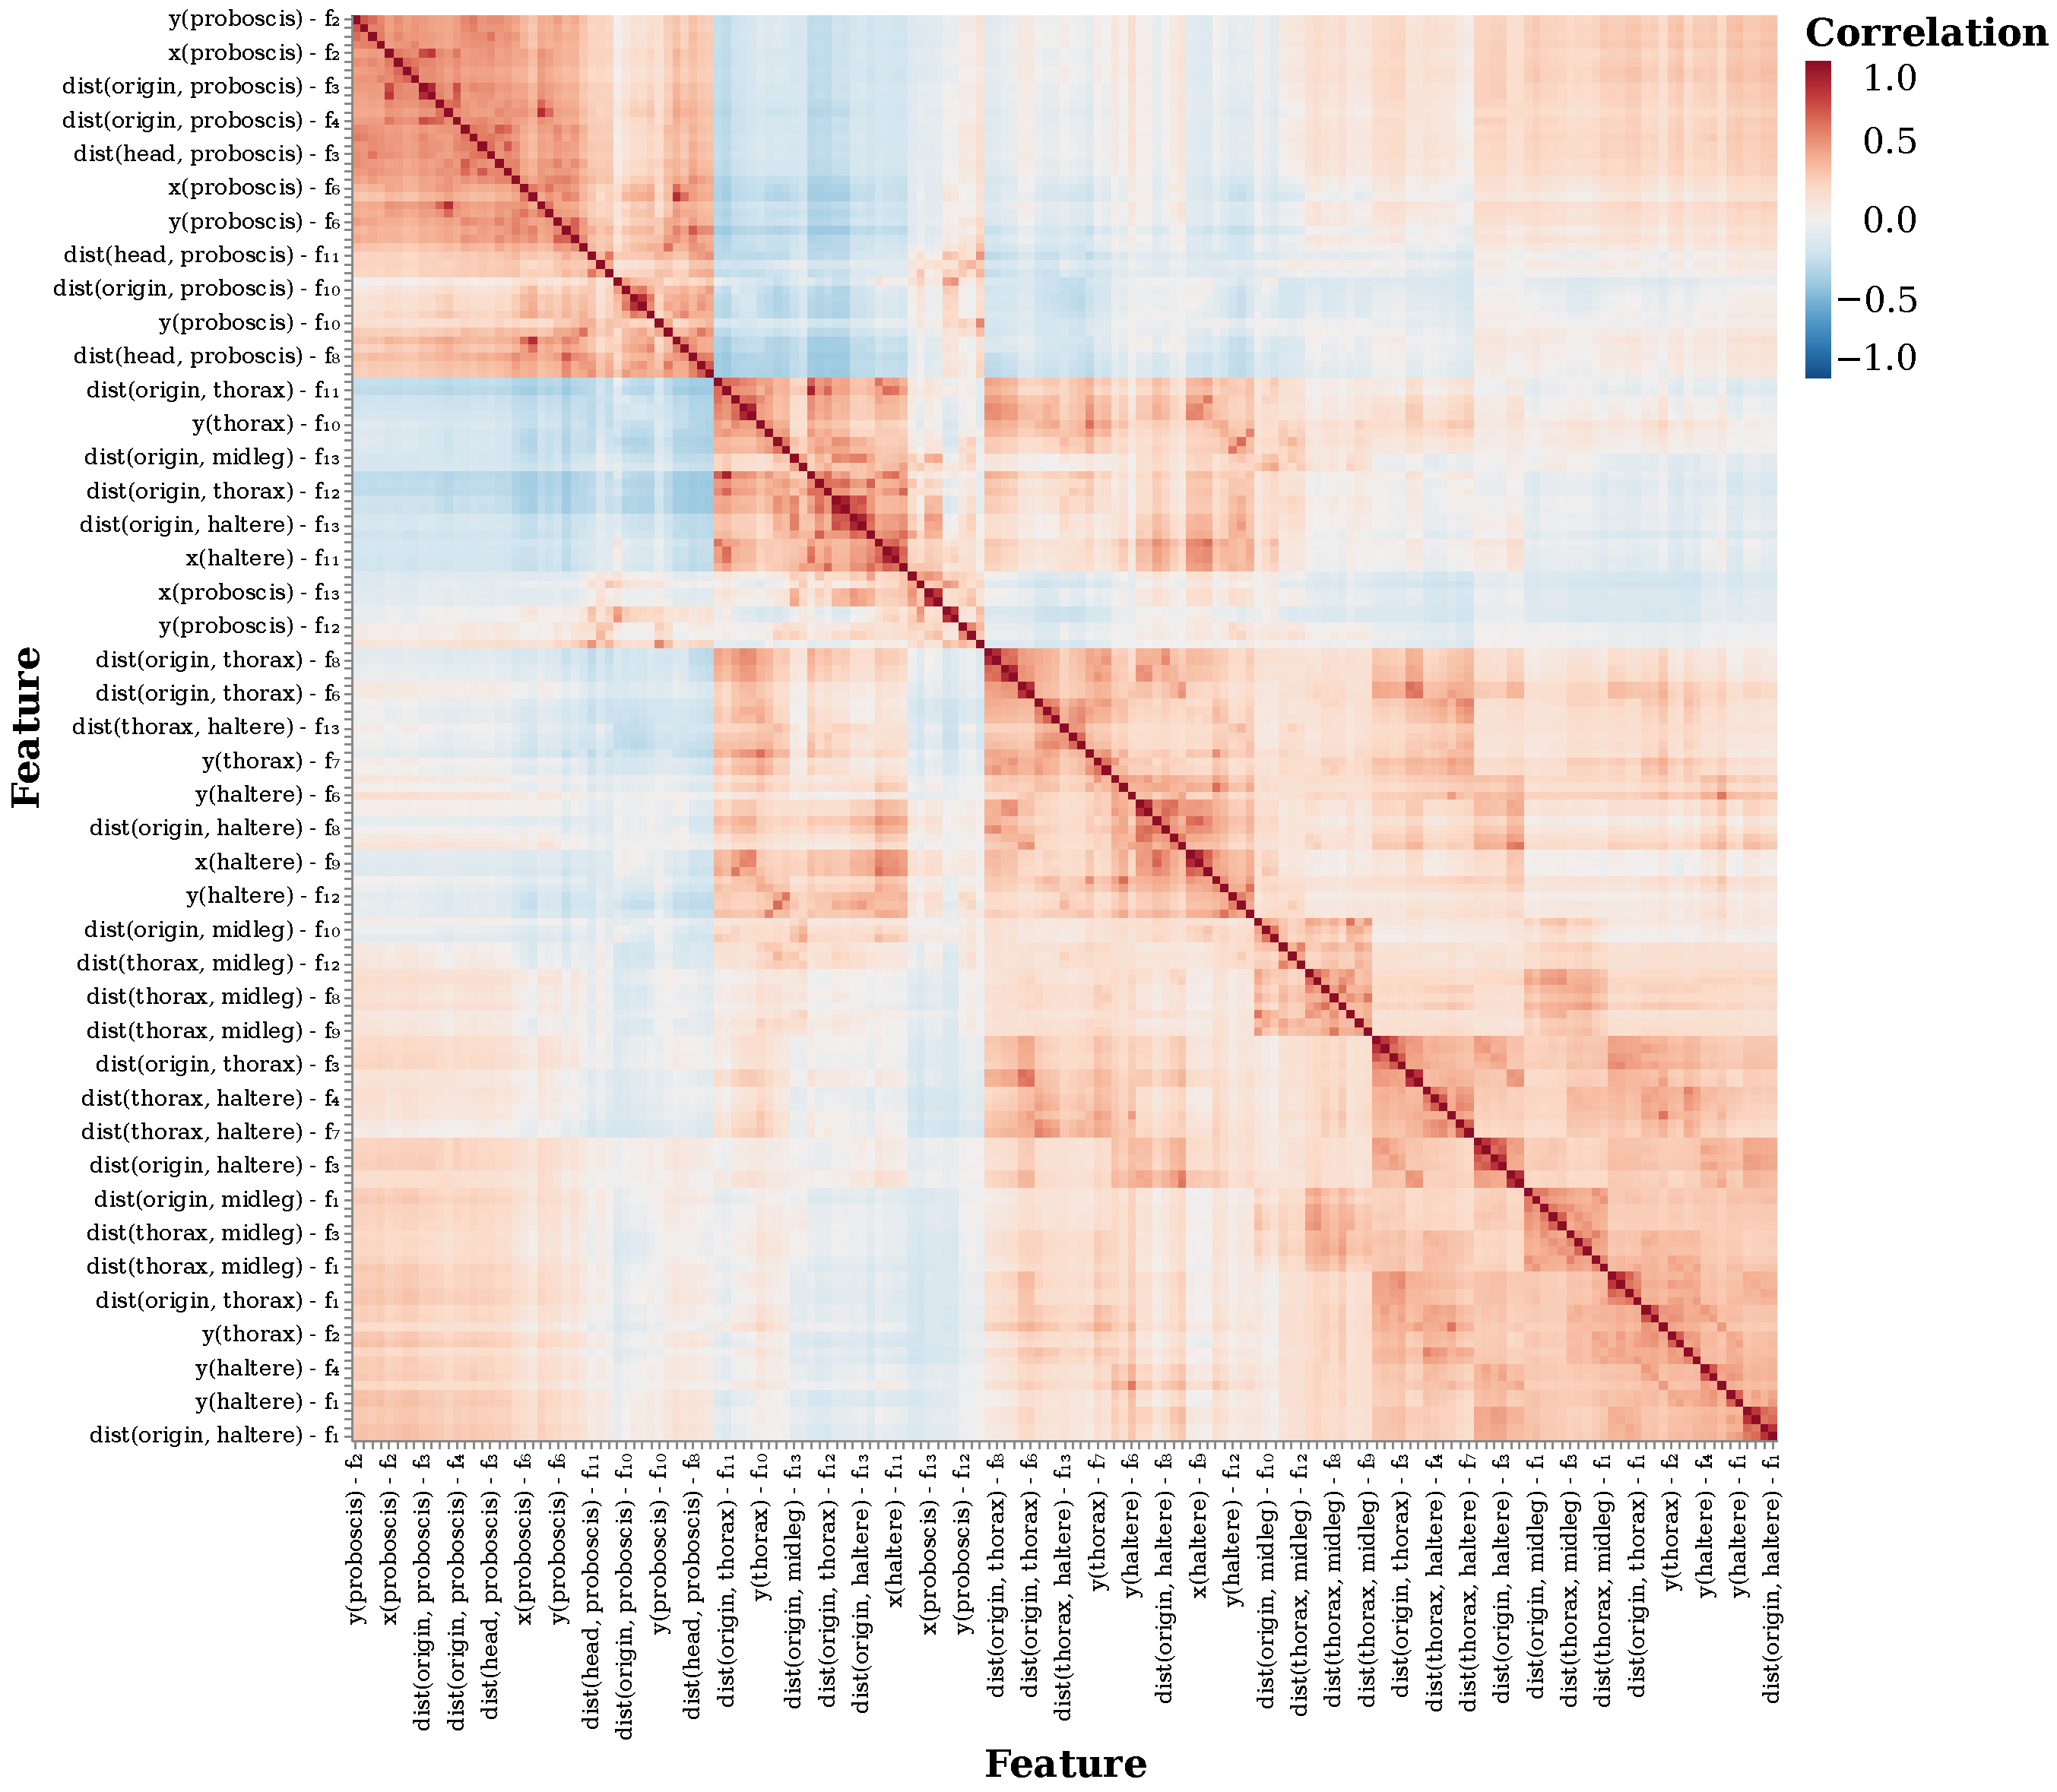
\includegraphics[width=0.70\linewidth]{figures/FeatureCorrelations-FlyF1DAnn-XY_labels.pdf}
	\caption[Spearman's correlation coefficient between each feature value of behavioral representations.]{Spearman's correlation coefficient between each feature value of behavioral representations. Features are clustered and grouped based on the absolute value of the correlation values. Frequency channels $f_1, \cdots, f_20$ are dyadically spaced between $1$ Hz and $20$ Hz. \label{figure:correlations-btw-features}}
\end{figure}

Many dimensionality reduction algorithms seek to preserve the pairwise distance structure among all the data samples, the well-known examples of such algorithms are PCA \citep{hotelling_analysis_1933}, and MDS \citep{kruskal_multidimensional_1964}.
Alternatively, some algorithms favor the preservation of local distances over global distance, such as UMAP (Uniform Manifold Approximation \& Projection) \citep{mcinnes_umap_2020} t-SNE \citep{maaten_visualizing_2008}, Laplacian Eigenmaps \citep{belkin_laplacian_2003} and LargeVis \citep{tang_visualizing_2016}.
The latter category of algorithms aims to achieve to preserve important local structures and helps to improve classification performance when used in combination with learning algorithms where the function is only approximated locally, e.g., $k$-nearest neighbor classifier \citep{mcinnes_umap_2020}.
Similarly, it has been shown that manifold learning based dimensionality reduction algorithms can improve the clustering performance \citep{sainburg_parametric_2021}.
Moreover, the trade-off of preserving local distances over global distances does not introduce any significant disadvantages in the latter stages of the behavioral pipeline.

We use UMAP for its superior performance in many aspects.
\citet{mcinnes_umap_2020} demonstrates that a $k$-nearest neighbor classifier trained on UMAP embeddings achieves higher accuracy for large $k$ values, compared to PCA, t-SNE, LargeVis, and Laplacian Eigenmaps since it captures non-local scales in a markedly effective way and local scales comparably or better.
Thus, it can be argued that UMAP has captured more of the global and topological structure of the benchmark datasets than its counterparts, t-SNE and LargeVis.
Another reason for choosing UMAP over other alternatives is that it tends to produce more stable embeddings.
It is capable of producing sub-sample embeddings that are very close to the full embedding even for sub-samples of $5\%$ of the dataset, outperforming the results of t-SNE and LargeVis.
Finally, the computational performance of UMAP scales well with the number of samples, the embedding dimensionality, and the data dimensionality, compared to t-SNE LargeVis, and Eigenmaps, resulting in significantly lower run-times on various datasets such as  COIL-20 \citep{nene_columbia_1996}, Fashion-MNIST \citep{xiao_fashion-mnist_2017}, and GoogleNews \citep{mikolov_distributed_2013}.
Run-time performance of the dimensionality reduction algorithm is an important concern in the behavioral mapping pipeline, as the number of samples and the data dimensionality is often on the order of $10^6$ and $10^2$, respectively.

UMAP and other non-linear dimensionality reduction algorithms that attempt to use a mathematical structure akin to a $k$-nearest neighbor graph to approximate a manifold, follow a similar basic structure as below \citep{mcinnes_umap_2020}.
\begin{itemize} \item Graph Construction \begin{enumerate}
		      \item Construct a weighted $k$-nearest neighbor graph.
		      \item Apply some transformation on the edge weights to envelop local distances.
		      \item Deal with the incompatibility of the local metrics, i.e., disagreeing weights of the edges.
	      \end{enumerate}
	\item Graph Layout
	      \begin{enumerate}
		      \item Define an objective function that preservers desired characteristics of the $k$-nearest neighbor graph.
		      \item Compute a low dimensional representation by optimizing the defined objective function.
	      \end{enumerate}
\end{itemize}

A distance metric is needed to construct a $k$-nearest neighbor ($k$-NN) graph.
In our case, we normalized the feature matrices as described in Section~\ref{section:feature-normalization}, feature vector entries at each time step sum up to $1$, and therefore the feature vectors  can be considered as discrete probability distributions.
We use the Hellinger distance \citep{hellinger_neue_1909} to quantify the similarity between ``discrete probability distributions'' of features, which is given by
\begin{equation}\label{equation:hellinger-distance}
	\operatorname{Hellinger}(P,Q)={\frac {1}{\sqrt {2}}}\;{\sqrt {\sum _{i=1}^{k}({\sqrt {p_{i}}}-{\sqrt {q_{i}}})^{2}}}.
\end{equation}
Then, based on the Hellinger distances, UMAP constructs a weighted $k$-NN graph using nearest neighbor descent \citep{dong_efficient_2011}.
Then, the $k$-NN graph is modified by making edges directed and defining the new weights using the local Riemannian metric of each data point.
After this step, there exist two edges with disagreeing weights between the nearest neighbors, as the local metrics differ.
UMAP combines those weights by using $t$-conorm and the resulting weight can be interpreted as the probability of at least one of the two directed edge to exist.

Finally, UMAP uses a force-directed graph layout algorithm in low dimensional space where attractive and repulsive forces are defined based on the gradients, optimizing the edge-wise cross-entropy between the original weighted graph and equivalent weighted graph induced by the embeddings.
The algorithm proceeds by iteratively applying attractive and repulsive forces at each edge or vertex.
Since the ``true'' graph captures the topology of the source data, the approximated graph also matches the overall topology of the data, and thus produces a meaningful low-dimensional representation.
A detailed mathematical and algorithmic description of the UMAP algorithm can be found in \citep{mcinnes_umap_2020}, and it is skipped here as it goes beyond the scope of this work.

\begin{comment}
\begin{algorithm}[!htbp]
	\caption{The main UMAP algorithm.}\label{alg:umap}
	\begin{algorithmic}[0]
		\setlength\baselineskip{18pt}
		\Function{UMAP}{$X$, $n$, $d$, min-dist, n-epochs}
		\State
		\State \# \textit{Construct the relevant weighted graph}
		\ForAll{$x \in X$}
		\State fs-set[$x$] $\gets$ \Call{LocalFuzzySimplicialSet}{$X$, $x$, $n$}
		\EndFor
		\State top-rep $\gets \bigcup_{x\in X} \textrm{fs-set}[x]$ \Comment{The probabilistic t-conorm is recommended.}
		\State
		\State \# \textit{Perform optimization of the graph layout}
		\State $Y \gets$ \Call{SpectralEmbedding}{top-rep, $d$}
		\State $Y \gets$ \Call{OptimizeEmbedding}{top-rep, $Y$, min-dist, n-epochs}
		\State \Return $Y$
		\EndFunction\vskip9pt
	\end{algorithmic}
\end{algorithm}
\end{comment}

The algorithm described above is an unsupervised method, but it can be easily extended to work in a supervised or semi-supervised manner.
Although we use a useful metric, e.g., Hellinger distance, defining the distance between a set of points, one can also define a simple metric for categorical values to extend UMAP further for supervised and semi-supervised cases.
We can obtain a second view of the source data by using a metric where distances for points in the same  and different categories as well as points without a category (for the semi-supervised case) are defined appropriately.
A straightforward and simple example would be defining distances as follows: 1 if the points are in the same category, 0 if the points are in different categories, and 0.5 if either of the points is uncategorized.
One can combine weighted graphs constructed using the two distance metrics (local metric and defined metric for categorical values), and arrive at a shared view of the data.
In the behavioral mapping pipeline, we benefit from unsupervised UMAP, and its supervised and semi-supervised extensions for different purposes.

The utilized behavioral embeddings fall into three different categories, namely ``disparate embeddings'', ``joint embeddings'' and ``pair embeddings'', detailed descriptions and their applications are described respectively in  Section~\ref{section:disparate-embeddings}, Section~\ref{section:joint-embeddings}, and  Section~\ref{section:pair-embeddings} respectively.

The resulting behavioral embedding
\begin{equation}
	\V{E}=\qmatrix{\V{e}_1, \cdots \V{e}_{F}} \in F \times N,
\end{equation}
is a low-dimensional representation of
\begin{equation}
	\mathrm{row}_{t_f} \V{\hat{W}} \in \mathbb{R}^{F \times \rbr{ N_S\card*{\mathcal{T}_S}}} \ \rbr{t_f \in \MicroActivity},
\end{equation}
where and $N << \rbr{ N_S\card*{\mathcal{T}_S}}$ and $F$ is the numbers of frames estimated as dormant and active, being equal to $\card{\MicroActivity}$.
Each frame $f$, corresponds to a time point $t_f\in \MicroActivity$.

\subsection{Disparate Embeddings}\label{section:disparate-embeddings}
UMAP may be used to embed high-dimensional behavioral representations of each experiment separately to obtain disparate behavioral embeddings. Treating each experiment separately is useful for several purposes.

For example, using supervised UMAP for annotated experiments, we can explore behavioral sub-categories in annotations as annotations are very high-level, biased and general categorization of behaviors. For instance, one annotation category, e.g., "grooming", can be consisted of two different clusters in the behavioral embedding space, corresponding to "grooming of head" and "grooming of abdomen" (see Figure~\ref{figure:supervised-disparate-zoomin-annotations}).
Defining very specific and low-level behavioral categories is not feasible and prone to error, a post-annotation analysis using disparate embeddings helps us to zoom in on annotated behaviors.
Another scenario of benefiting disparate embeddings is using unsupervised UMAP for annotated and/or unannotated experiments separately.
We can visualize how behavioral repertoire is represented in the low-dimensional embeddings space and analyze which features drive different regions and clusters of the behavioral embeddings (see Figure~\ref{figure:unsupervised-disparate-behavioral-regions}).

\begin{figure}[htb!]
	\centering
	\begin{subfigure}[b]{0.5\linewidth}
		\centering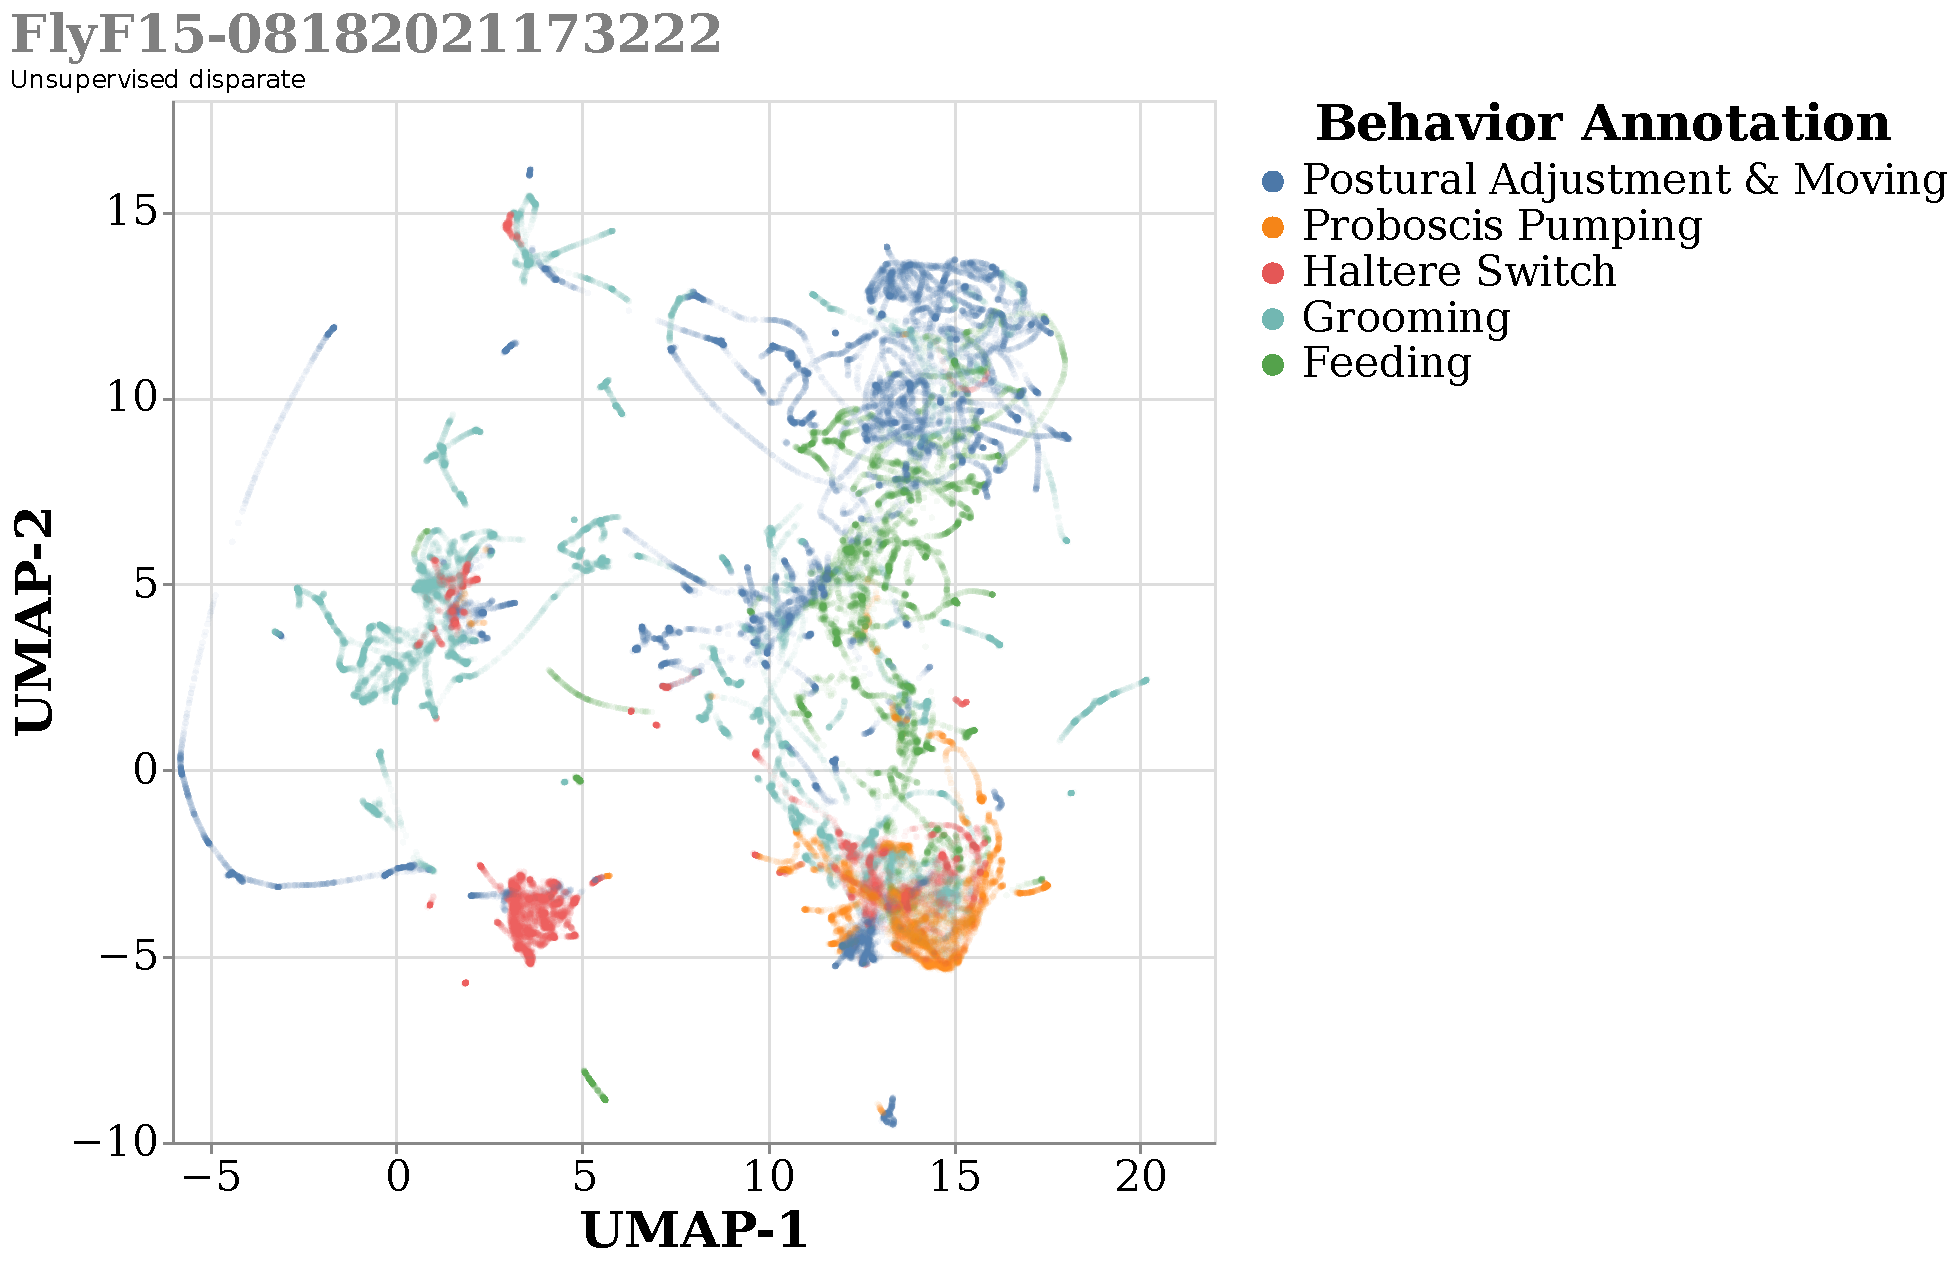
\includegraphics[height=5cm]{figures/FlyF15-08182021173222_UnsupervisedDisparateEmbedding.pdf}
		\caption{Unsupervised. \label{figure:unsupervised-disparate-behavioral-regions}}
	\end{subfigure}%
	\hfill
	\centering
	\begin{subfigure}[b]{0.5\linewidth}
		\centering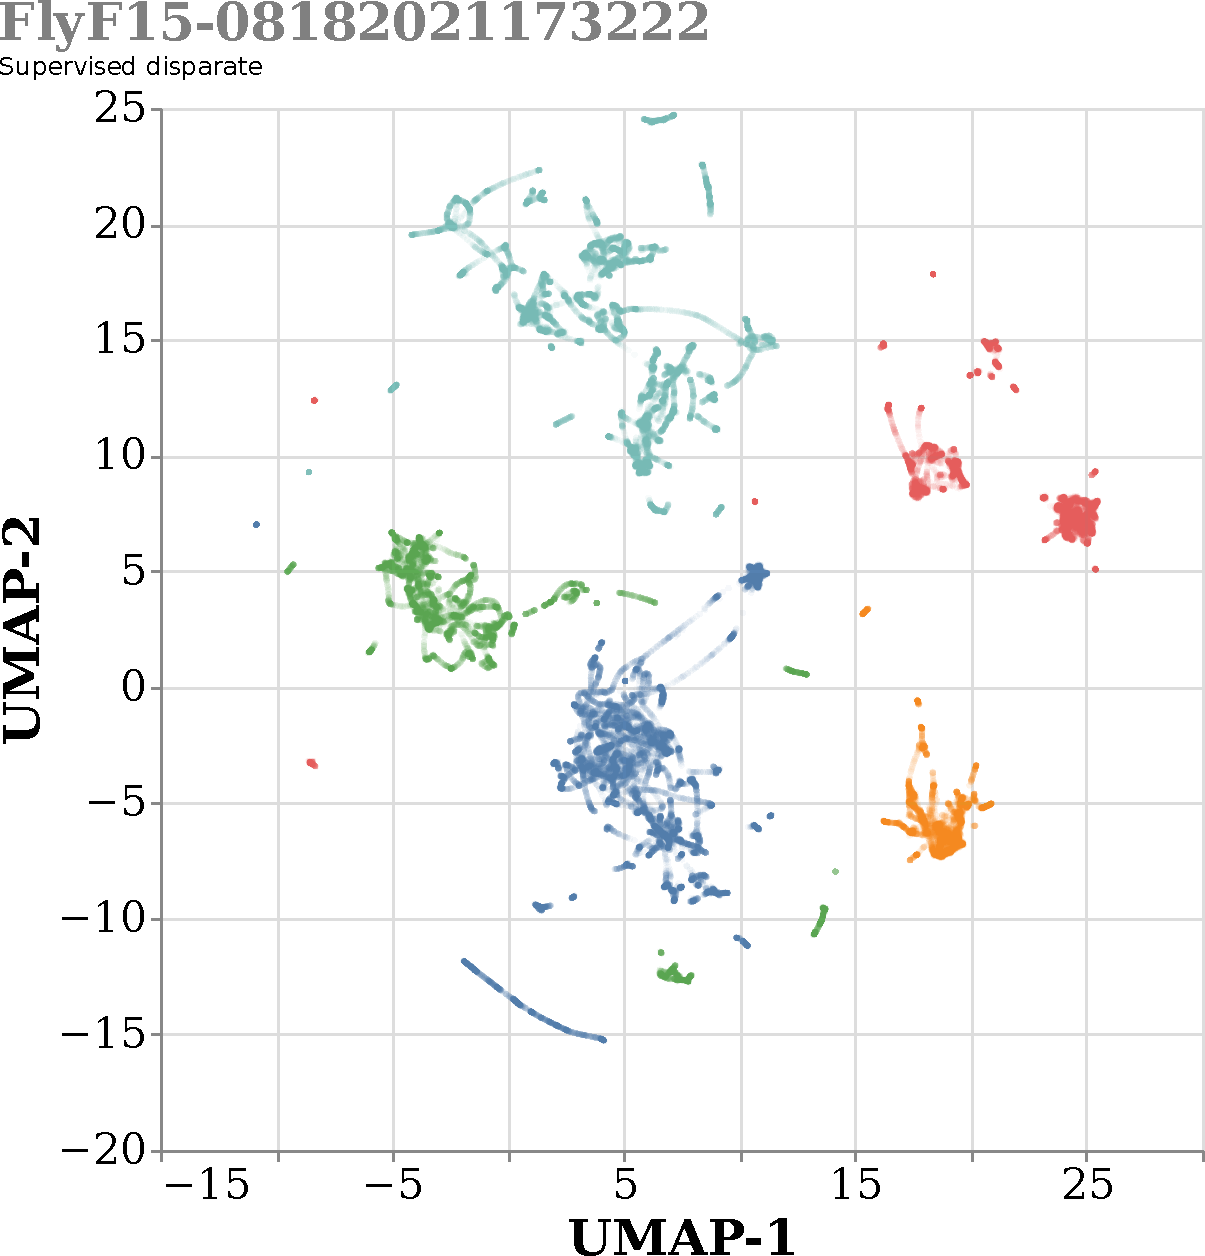
\includegraphics[height=5cm]{figures/FlyF15-08182021173222_SupervisedDisparateEmbedding.pdf}
		\caption{Supervised. \label{figure:supervised-disparate-zoomin-annotations}}
	\end{subfigure}%
	\caption[Supervised and unsupervised embeddings of FlyF15-08182021173222.]{Two-dimensional supervised and unsupervised behavioral embeddings of FlyF15-08182021173222. Both embeddings reveal variations within annotated behavioral categories.}
\end{figure}

\subsection{Joint Embeddings}\label{section:joint-embeddings}
Ideally, we would like to embed all experiments into a shared joint behavioral space, and using such an embedding would enable us to discover stereotypical and common behaviors among different flies.
However, we observed that this is only possible to a certain extent and such joint embeddings tend to not mix well as the number of experiments increases.
When we jointly compute a behavioral space using all available experiments,  the resulting embedding is usually not totally homogeneous in terms of flies and experiments.
We observed that similar behaviors might end up embedded in different regions, and multiple clusters consisting of highly similar behaviors emerge.

Especially for the joint treatment of annotated experiments, supervised UMAP fails to embed similar behaviors of different experiments closely and homogeneously.
There are many factors contributing to this impairment of supervised joint embeddings, such as behavioral variations among flies and experiments,  differences in orientation while exhibiting similar behaviors, and broad definitions of annotation categories.
Unless the number of jointly embedded experiments does not exceed several, unsupervised UMAP performs relatively well, and enables a fully unsupervised and unbiased analysis of behaviors.
We can exploit unsupervised joint behavioral embeddings for visualization purposes to discover how different feature combinations are exhibited, and density-based clustering to extract similar behavioral bouts.
However, utilizing unsupervised joint embeddings becomes problematic as the number of experiments increases, and behavioral space gets ``too crowded''.

\subsection{Pair Embeddings}\label{section:pair-embeddings}
Using disparate embeddings does not allow one to embed an annotated and an unannotated experiment into a joint behavioral space, and joint embeddings poorly blend different experiments in a shared space.
Instead, we propose a novel alternative approach to benefit from the semi-supervised dimensionality reduction capabilities of UMAP, while avoiding generating a hard-to-interpret embedding.
In this approach, namely semi-supervised pair embeddings, we compute a joint behavioral space for each annotated and unannotated pair, using the available annotations.
As a result, for $\Unann{R}$ unannotated experiments and  $\Unann{R}$ annotated experiments, a semi-supervised pair embedding will be generated for each $\Unann{R} \times \Ann{R}$ pair.

For a single unannotated experiment, a semi-supervised behavioral embedding for each annotated experiment provides different ``views''.
Especially when the behavioral repertoire of the annotated and the unannotated experiments are similar, the provided ``view'' turns out to be an accurate, easy-to-interpret low-dimensional representation of the exhibited behaviors of the unannotated experiment.
When the behavioral repertoire and/or feature distribution are dissimilar, the resulting embedding may not provide useful information about the unannotated experiment, but an advantage of this approach is that the other pair embeddings do not get distorted by poor matches.
As described in Section~\ref{section:nearest-neighbors-classification}, semi-supervised pair embeddings are utilized to predict behavioral categories of unannotated experiments by combining multiple view acquired from annotated ones.

\begin{figure}[htb!]
	\centering
	\begin{subfigure}[b]{0.5\linewidth}
		\centering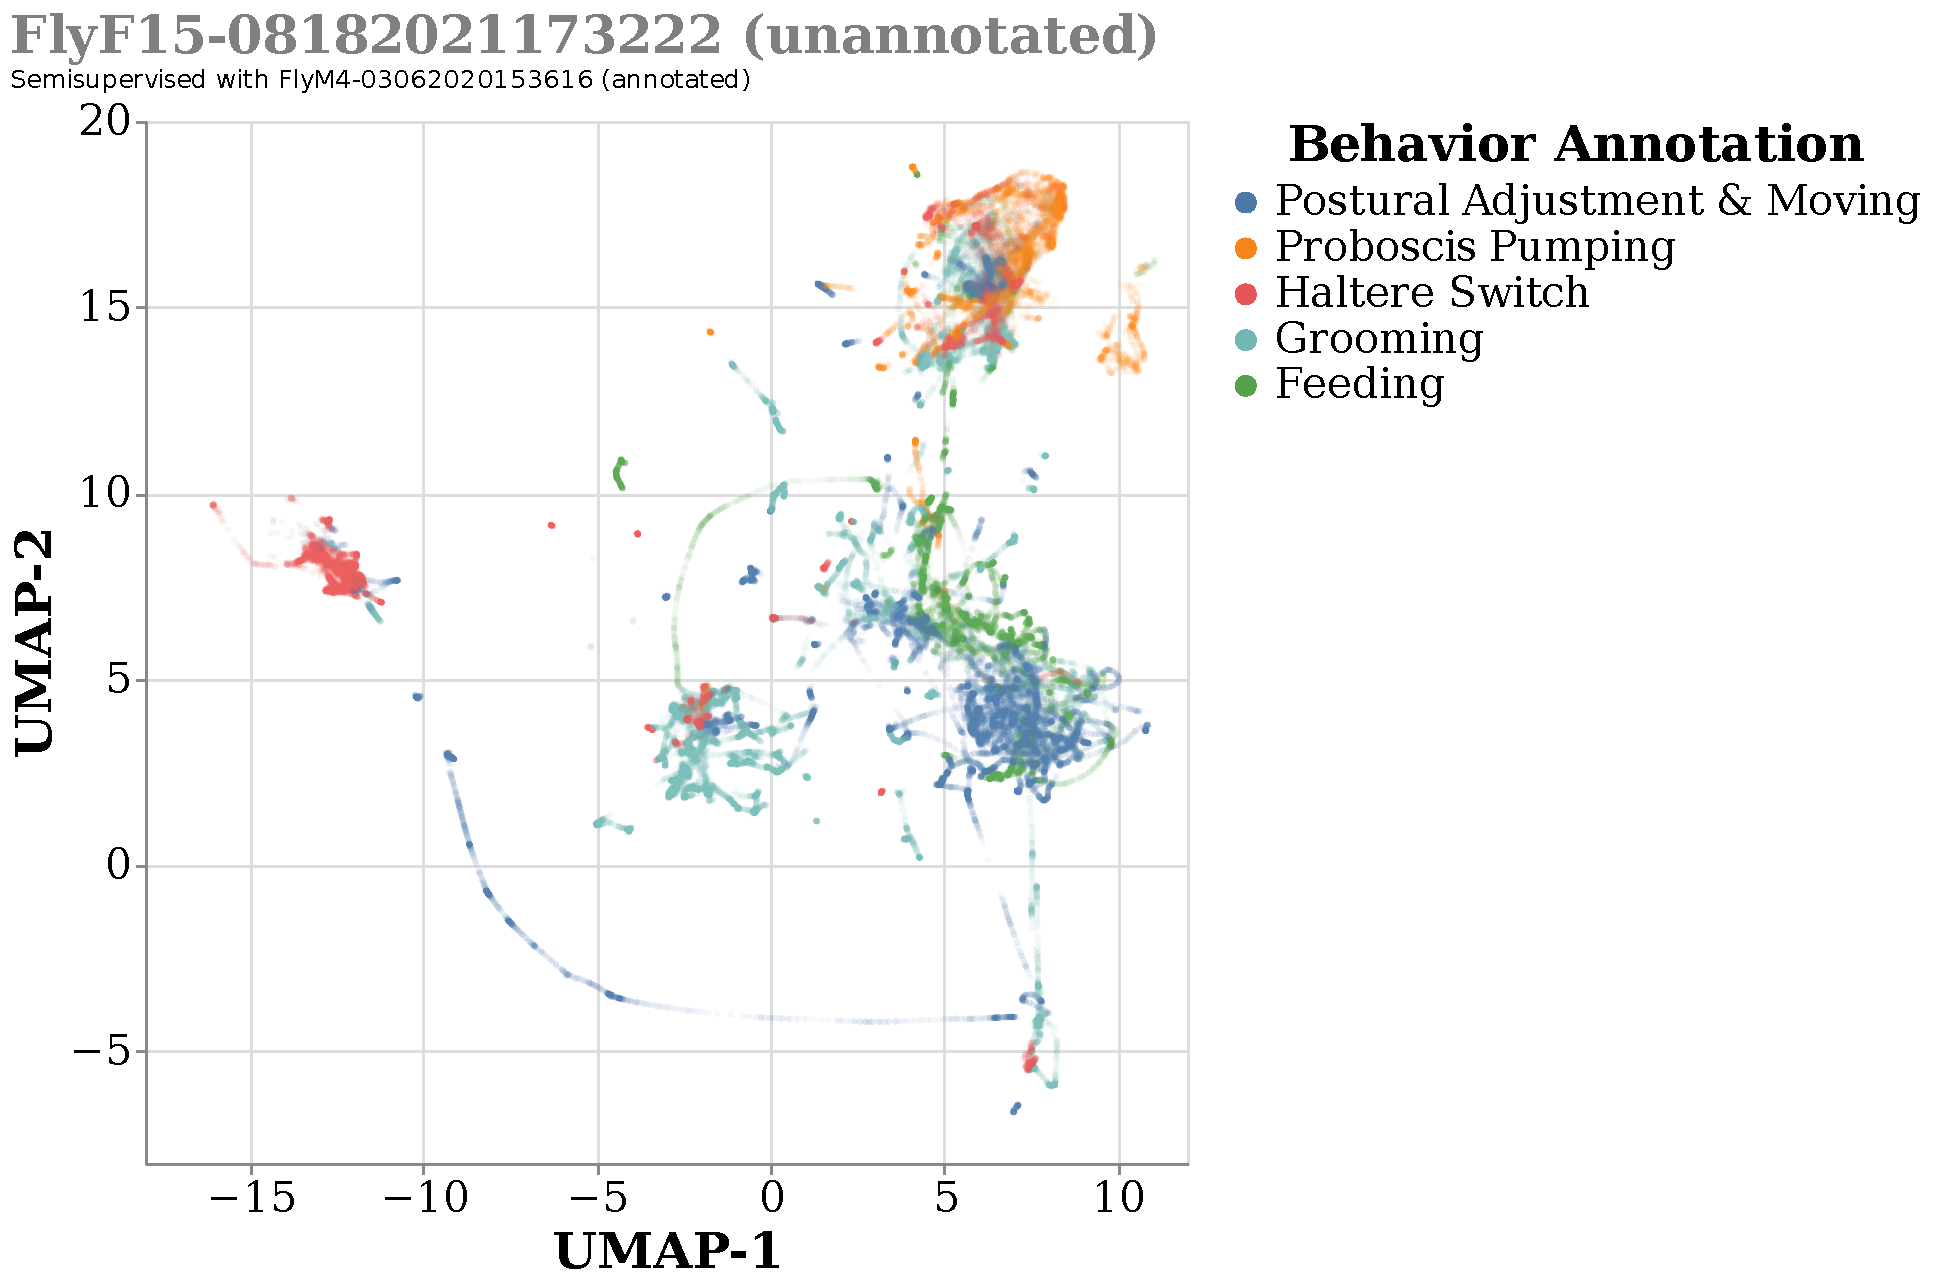
\includegraphics[height=5cm]{figures/FlyF15-08182021173222_FlyM4-03062020153616-SemisupervisedPairEmbedding.pdf}
		\caption{Only unannotated experiment.}
	\end{subfigure}%
	\hfill
	\centering
	\begin{subfigure}[b]{0.5\linewidth}
		\centering\includegraphics[height=5cm]{figures/FlyF15-08182021173222_FlyM4-03062020153616-SemisupervisedPairEmbedding-JointChart.pdf}
		\caption{Unannotated and annotated experiments.}
	\end{subfigure}%
	\caption[Semi-supervised pair embeddings with an annotated and an unannotated experiment.]{Semi-supervised pair embeddings with an annotated and an unannotated experiment. FlyM4-03062020 (annotated) provides a ``view'' on the behavioral repertoire of the FlyF15-08182021 (unannotated).}
\end{figure}

\begin{comment}
\section{Soft Clustering}
\citet{mcinnes_hdbscan_2017} \citet{campello_density-based_2013}
\NOTE{
	We always use soft clustering feature of HDBSCAN, since it is very beneficial to have a composite assignment for a data-point.
	For example, 0.7 grooming, 0.3 proboscis pumping may indicate that those two behaviors are simultaneously exhibited or a combination of both is exhibited etc.
	We can always take $\argmax$ if a categorical label is needed.
}

\subsection{Disparate Clustering}

\NOTE{
	If embedding is a disparate embedding, then we directly cluster each of them separately.
	If a joint embedding or pair embedding is clustered, then experiments need to be extracted from the embedding space first, and then they need to be clustered separately.
}

\subsection{Joint Clustering}
\NOTE{
	This is only applicable to joint and pair embeddings. We cluster all the experiments in the behavioral embedding together.
}

\subsection{Crosswise Clustering}
\NOTE{
	This is again only applicable to joint and pair embeddings.
	For joint embeddings, we exclude a subgroup of experiments.
	For pair embeddings, we exclude one of the pair experiments.
	Then rest of the embedding is clustered and clusters are formed.
	Finally, for each excluded embedding, soft cluster membership vectors are computed based on the formed clusters.
}

\subsection{Mapping Clusters to Behavioral Categories}
\NOTE{
	If a clustering contains annotated experiments, we map that clusters in that clustering to a behavioral composition as follows ({\it subject to change, there are couple of alternatives})
	\begin{equation}
		m_\alpha = \frac{\textnormal{number of frames with annotation }\alpha \textnormal{ in the cluster}}{\textnormal{total number of frames with annotation }\alpha}.
	\end{equation}
	So for each cluster, we end up with a vector $\mathbf{m}=(m_\alpha)$, represent it behavioral composition.
}
\NOTE{
	Behavioral score of unannotated experiment will be computed using clustering membership score and behavioral composition mapping of those clusters.
	For example, using semi-supervised pair embeddings and crosswise clustering; one can compute behavioral scores for a frame as follows;
	\begin{equation}
		y_\alpha = \sum_{c=0}^C m^c_\alpha
	\end{equation}
	where $C$ is the number of clusters, $\mathbf{m}^c$ is the behavioral composition of the cluster $c$.
	As a result, for each frame, we end up with a behavioral score vector $\mathbf{y}=(y_\alpha)$.
}
\end{comment}

\section{Nearest Neighbor Analysis and Classification}\label{section:nearest-neighbors-classification}
One of our ultimate goals is to annotate an experiment using already annotated ones.
In previous sections and chapters, we described feature extraction, activity detection, and computation of behavioral embeddings.
In this section, we describe a novel nearest neighbor based classification approach, which has to tackle the following challenges:
\begin{itemize}
	\item sparsity of behavioral expressions,
	\item imbalanced distribution of behavioral categories,
	\item scarcity of annotated experiments, which are laborious to produce,
	\item variation between experiments.
\end{itemize}
Our approach consists of two steps, briefly stated as follows:
\begin{enumerate}
	\item computing behavioral weights of an unannotated experiment, using its semi-supervised pair embeddings for each annotated  experiment,
	\item combining behavioral weights of the unannotated experiment with an annotated experiment committee by voting.
\end{enumerate}
We compute the behavioral weights with our nearest neighbor based approach by considering the sparsity of behavioral expressions and imbalanced distribution of behavioral categories, as described in Section~\ref{section:behavioral-weights}.
In Section~\ref{section:committee-by-voting}, we detail the committee-by-voting approach, which helps us to deal with variation between experiments by providing multiple ``views'' on observed behavioral expressions that we attempt to annotate. Finally, the post-processing of resulting predictions is described in Section~\ref{section:postprocessing-predictions}.

\subsection{Behavioral Weights}\label{section:behavioral-weights}
Consider two experiments, an annotated one $\exptAnn$, and an unannotated one $\exptUnann$, and their semi-supervised pair embedding, respectively $\Ann{\V{E}}=\qmatrix{\Ann{\V{e}}_1, \cdots \Ann{\V{e}_{\Ann{F}}}}$ and $\Unann{\V{E}}=\qmatrix{\Unann{\V{e}}_1, \cdots \Unann{\V{e}}_{\Unann{F}}}$.
Given the true annotations $\Ann{\V{y}}$ of the frames in the $\Ann{\MicroActivity}$ set of $\exptAnn$, and $K$ behavioral categories, the goal is to compute $\V{\hat{b}}_f=\qmatrix{\hat{b}_{f,1}, \cdots \hat{b}_{f,K}}$, representing the weights (in other words, the similarity score) of each behavioral category for $\exptUnann$, using $\Ann{\V{E}}, \Unann{\V{E}}$ and $\Ann{\V{y}}$.

The procedure start by querying $k$-nearest neighbors of $\exptUnann$'s each frame $f$ in the joint behavioral embedding space consisting of $\Ann{\V{E}}$ and $\Unann{\V{E}}$, using the $k$-d trees for efficiency \citep{bentley_multidimensional_1975}. $\NN{k}{f}$ denotes the set of indices of $\Unann{\V{e}}_f$'s $k$ nearest neighbors, and the $k$-NN weight $b_{f,i}$ for each query point (i.e., frame) $f$ of $\exptUnann$, and behavioral category $i$, is computed by
\begin{equation}\label{equation:nn-weights}
	b_{f,i} = \begin{dcases}
		\sum_{f^\prime \in \NNi{k}{i}{f}}\frac{1}{\dist{\Unann{\V{e}}_f}{\Ann{\V{e}}_{f^\prime}}^p + \epsilon} & \textnormal{if } \card{\NNi{k}{i}{f}} \neq 0, \\
		0                                                                                                      & \textnormal{if otherwise},
	\end{dcases} \qbwhere p \in \set{0,1,2}.
\end{equation}
Here, $\NNi{k}{i}{f}=\Set{f^\prime}{\Ann{y}_{f^\prime}=i, \dband f^\prime \in \NN{k}{f}}$, is the set of indices of data points of $\exptAnn$ whose annotation is the behavior category $i$ and is one of the $k$ nearest neighbors of $\Unann{\V{e}}_f$.
$\dist{\Unann{\V{e}}_f}{\Ann{\V{e}}_{f^\prime}}$ is the euclidean distance between $\Unann{\V{e}}_f$ and $\Ann{\V{e}}_{f^\prime}$, and $p$ parameterizes the relation between distance and weight $b_{f,i}$.
We add a small number $\epsilon$ ($10^{{-}6}$) to the denominator to avoid numerical errors.
The resulting vector $\V{b}_f = \qmatrix{b_{f,1}, \cdots, b_{f,K}}$ weights the similarity of the frame $f$ to each behavioral category in the shared embedding space based on nearest neighbors.

Naturally, the number of occurrences or durations of the behavior bouts are different for each behavioral category, and therefore, $\Ann{\V{y}}$ is highly imbalanced.
As a result, the number of nearest neighbors and $\V{b}_f$ are biased in favor of frequently occurring and long-bout behaviors.
For instance, pumping-like movements of the proboscis occur more frequently in longer bouts than switch-like movements of the haltere.
Especially when $k$ is large, it becomes crucial to consider the imbalanced distribution of behavior occurrences, since the embedding space will be dominated by frequent behaviors.
Thus, incorporating this imbalance into the formulation may help to improve the recall of rarely occurring short-bout behaviors and precision of frequently occurring long-bout behaviors.
To achieve this, we normalize the scores previously computed, $b_{f,i}$, as a function of the number of occurrences of the behavioral category $i$ as follows:

\begin{equation}\label{equation:behavioral-weight-occurence-normalization},
	b^\prime_{f,i} = \frac{b_{f,i}}{\rbr{1 + N^{\plus}_i}^p} \qbor \frac{b_{f,i}}{\log_k(1 + N^{\plus}_i)} \qbwhere p \in \set{0, \sfrac{1}{2}, 1}, k \in \set{2, 10},
\end{equation}
where $N^{\plus}_i = \card*{\Set{f}{y^{\plus}_f=i}}$ is the number of frames annotated as behavioral category $i$.
In the above equation, two different alternatives are given for this normalization step; a polynomial one and a logarithmic one, where $p$ and $k$ parameterize the relation between $N^{\plus}_i$ and $b^\prime_{f,i}$.
For instance, if one is mostly interested in achieving high recall for frequently occurring behaviors, low $p$ values or using the logarithmic alternative might be more appropriate.
It may be even desired to set $p=0$, and not considering the number of occurrences in some cases, see Section~\ref{section:employing-proposed-pipeline} for more details.

The resulting vector $\V{b^{\prime}}_f \in \reals^K$ is dependent on the annotated experiment $\exptAnn$, and the vectors computed based on different annotated experiments are not comparable with each other.
Hence, we map the values of $b^\prime_{f,i}$ to $\sqbr{0,1}$ using either the $\operatorname {softmax}$ function or $\textnormal{L}_1$ normalization as follows:
\begin{equation}\label{equation:behavioral-weight-activation}
	\hat{b}_{f,i} = \frac{\exp{b^\prime_{f,i}}}{\sum_{j=1}^{K} \exp{b^\prime_{f,j}}} \qbor \frac{b^\prime_{f,i}}{\sum_{j=1}^{K} b^\prime_{f,j}}.
\end{equation}
The resulting behavioral weight vector $\V{\hat{b}}_f \in \sqbr{0,1}^K$ can be considered as a probability distribution.
Here, the vector $\V{\hat{b}}_f$ represents the behavioral characteristics of the frame $f$ of $\exptUnann$ based on the behavioral repertoire of $\exptAnn$.
The voting-like scheme, as described in Section~\ref{section:committee-by-voting}, incorporates the behavioral weight vectors of all annotated experiments to finalize the classification for $\exptUnann$.

\subsection{Experiment Committee by Voting}\label{section:committee-by-voting}
Consider all experiments: unannotated experiments $\exptUnann_1, \cdots, \exptUnann_{\Unann{R}}$, and annotated experiments $\exptAnn_1, \cdots, \exptAnn_{\Ann{R}}$, where $\Unann{R}$ and $\Ann{R}$ are the number of experiments, respectively.
The goal is to combine the behavioral weights of an unannotated experiment $\exptUnann_k$, calculated separately for each annotated experiment.

Let $\V{\hat{b}}_f^{k,l}$ denote the behavioral weights of $\exptUnann_k$ computed with $\exptAnn_l$.
Each annotated experiment contributes to the overall behavioral score of $\exptUnann_k$; in other words, annotated experiments, forming a committee,  vote according to $\V{\hat{b}}_f^{k,l}$.
Each annotated experiment provides a different view of the behavioral repertoire, as in the case of pair embeddings (see Section~\ref{section:pair-embeddings}).
Before describing hard voting and soft voting approaches, there is one more step to discuss.

There exists a significant variation among the exhibited behavioral repertoires in the experiments.
An annotated experiment might lack some behavioral expressions or manifest some behaviors excessively.
In such cases, if the behavioral weight vector $\V{\hat{b}}_f^{k,l}$ is not confident, i.e., weights of behavioral categories are close to each other, one may want to decrease its contribution to the voting.
To achieve this, we propose two optional approaches; penalizing the behavioral weights with the entropy of the ``probability distribution'' $\V{\hat{b}}_f^{k,l}$, or with the uncertainty.
The contribution of votes of $\exptAnn_l$ to the committee formed for $\exptUnann_k$ is $\Vvote_f^{k,l} = \qmatrix{\vote_{f,1}^{k,l}, \cdots, \vote_{f,K}^{k,l}}$, and is given by
\begin{equation}
	\vote_{f,i}^{k,l} = \rbr{\log_2(K) - \entropy{\V{\hat{b}}_f^{k,l}}} \hat{b}_{f,i}^{k,l} \qbor \rbr{ 1 - \max_{1 \leq j \leq K} \hat{b}_{f,j}^{k,l}} \hat{b}_{f,i}^{k,l} \qbor \hat{b}_{f,i}^{k,l}.
\end{equation}
If $\max_i \hat{b}_{f,i}$ is close to $\sfrac{1}{K}$, which means that the computed vector weights the behaviors uniformly, then the factors $\rbr{\log_2(K) - \entropy{\V{\hat{b}}_f^{k,l}}}$ or $\rbr{ 1 - \max_{1 \leq j \leq K} \hat{b}_{f,j}^{k,l}}$ may be used to decrease the ``importance'' of the vote.

Now, after computing behavioral votes for each annotated and unannotated experiment pair, we can combine those votes for a single unannotated experiment $\exptUnann_k$  by forming a committee of annotated experiments $\exptAnn_1, \cdots, \exptAnn_{\Ann{R}}$.
The predicted behavioral category at frame $k$ of $\exptUnann_k$ is given by the combined votes of the committee.
The predicted behavioral category at frame $k$ of $\exptUnann_k$, denoted by $\hat{y}^k_f$, is given by combined votes of the committee.
To obtain the overall aggregate view of the committee, we can follow two alternative voting schemes, namely hard voting (i.e., majority rule voting) or soft voting.
At this point, we may want to have scores for each behavioral category rather than hard labels.
Such score information might be desired to capture the complex and hierarchical structure of the behaviors.
Behaviors sometimes occur simultaneously, and sometimes observed behaviors might manifest similarities to more than one behavioral category \citep{berman_predictability_2016}.
Hence, one may also use the combined vote scores directly, without computing the $\argmax$.

\subsubsection{Hard Voting}
In the hard voting scheme, the prediction of a frame $f$ is given by the majority behavioral category of the $\argmax$ of each annotated experiment's votes and computed by the following formula:
\begin{equation}
	\hat{y}^k_f = \argmax_{1 \leq i \leq K} \Set{\argmax_{1 \leq j \leq K} { \vote_{f,j}^{k,l}}}{j=i, \, 1 \leq l \leq \Ann{R}}.
\end{equation}

\subsubsection{Soft Voting}
In contrast to majority voting (hard voting), the soft voting scheme assigns the behavioral category as the $\argmax$ of the sum of each annotated experiment's vote vector, and $\hat{y}^k_f$ is given by
\begin{equation}
	\hat{y}^k_f = \argmax_{1 \leq i \leq K} \sum_{l=1}^{\Ann{R}} \vote_{f,i}^{k,l}.
\end{equation}

\subsubsection{Behavioral Scores}
Definitions of behavioral categories might be broad, and expressed behaviors sometimes are a combination of multiple behavioral categories.
For example, a switch-like movement of the haltere can simultaneously occur with a postural adjustment.
One may also want to examine and interpret top-$k$ predictions, especially when there exist many narrow behavioral categories.
Thus, in addition to assigning categories to frames, it is also useful to compute and report scores for behavioral categories based on the votes contributed by each annotated experiment.
Moreover, such scores can be utilized as confidence scores and might be helpful to analyze differences in the behavioral repertoire (see Figure~\ref{figure:behavioral-score-distributions} and Figure~\ref{figure:repertoire-difference}).

For a behavioral category $i$, such a score can be calculated by combining votes as follows:
\begin{equation}
	\frac{\sum_{l=1}^{\Ann{R}} \vote_{f,i}^{k,l}}{\sum_{i = 1}^{K}\sum_{l=1}^{\Ann{R}} \vote_{f,i}^{k,l}}.
\end{equation}

\subsection{Post-processing}\label{section:postprocessing-predictions}
Finally, we post-process predicted annotations to improve our nearest neighbor based algorithm by incorporating a couple of assumptions on the temporal organization of the behaviors and physical constraints.
Before applying post-processing procedures, the frames in the sets $\MacroActivity$ and $\Quiescence$ should be recovered, as we only predicted the annotations of the frames in the set $\MicroActivity$.
Without having a temporally continuous vector of annotations, post-processing would lead to unintended consequences and erroneous results.
Let $\VpredAnn^k=\rbr{\hat{y}^k_1, \cdots, \hat{y}^k_T}$ be the $\exptUnann_k$'s vector of predicted annotations for the entire experiment, defined as follows:
\begin{equation}
	\predAnn^k_t =
	\begin{cases}
		0           & \textnormal{if } t \in \Quiescence_k,                             \\
		\hat{y}^k_f & \textnormal{if } t \in \MicroActivity_k \textnormal{ and } t=t_f, \\
		K+1         & \textnormal{if } t \in \MacroActivity_k.
	\end{cases}
\end{equation}
This vector of annotations spans an entire experiment of $k$ and consists of detailed annotations of behavioral subcategories during dormancy, the general category of macro-activities, and quiescence.

Before discussing post-processing, we first need to define behavioral bouts.
Informally, a behavioral bout is a segment of time, in which the same behavioral category is continuously observed.
We can formally define a behavioral bout for a given $\hat{y}^k_t$ as follows:
\begin{equation}
	\begin{aligned}
		\mathsf{bout}^0_t & =\max\cbr{{\argmax_{t^\prime} \rbr{\hat{y}^k_t \neq \hat{y}^k_{t^\prime}} \land \rbr{1 \leq t^\prime \leq t} \lor \rbr{t^\prime = 1}}}, \\
		\mathsf{bout}^1_t & =\min\cbr{{\argmax_{t^\prime} \rbr{\hat{y}^k_t \neq \hat{y}^k_{t^\prime}} \land \rbr{t \leq t^\prime \leq T} \lor \rbr{t^\prime = T}}},
	\end{aligned}
\end{equation}
where $\mathsf{bout}^0_t$ and $\mathsf{bout}^1_t$ are respectively the beginning and the end of the behavioral bout, to which $\hat{y}^k_t$ belongs.

We have sensible expectations about the duration of behavioral bouts of each behavioral category acquired by human annotators.
For instance, a bout of proboscis's pumping-like movement should not be shorter than $200$ millisecond, as bout duration distributions of annotations indicate.
In addition to annotations, we may have reasons for physical and biological constraints.
An example is that grooming behavior, bout duration of grooming can not exceed a couple of minutes, probability of observing a grooming behavior lasted longer than $2$ minutes is extremely low \citep{qiao_automated_2018}.
Considering such constraints and temporal expectations, we apply the following post-processing procedures, and parameters should be determined based on the behavioral repertoire of interest.
Post-processing procedures are especially helpful for avoiding misleading classification of the time points with erroneous tracking of body parts.
Each procedure is optional but should be applied in the given order.

\subsubsection{Pruning Interrupting Bouts}\label{section:pruning-interrupting-bouts}
We prune short intervals interrupting possibly long and continuous behavioral bouts.
Given a window size $\tau$, the majority behavioral category in the surrounding window around a time point $t$ is assigned that point by:
\begin{equation}
	\hat{\predAnn^k_t} = \argmax_{\symsf{a}} \card{\Set{t^\prime}{\predAnn^k_{t^\prime}=\symsf{a}, \ \max\cbr{1, t-\tau} \leq t^\prime \leq \min\cbr{t+\tau, T}}}.
\end{equation}
The window size $\tau$ is typically less than a second.

\subsubsection{Elimination of Overly Long and Overly Short Bouts}
We eliminate behavioral bouts whose durations are extremely short or extremely long, and hence, contradict physical constraints and our temporal expectations.
For each behavioral category $i$, we define two thresholds $\delta^{\symrm{short}}_i$ and $\delta^{\symrm{long}}_i$, namely upper bound and lower bound.
Then, the behavioral bouts whose duration is longer or shorter than the corresponding thresholds, are set to quiescence.
\begin{equation}
	\hat{\predAnn}^k_t=
	\begin{cases}
		0            & \mathsf{bout}^0_t - \mathsf{bout}^1_t < \delta^{\symrm{short}}_{\predAnn^k_t}, \\
		0            & \mathsf{bout}^0_t - \mathsf{bout}^1_t > \delta^{\symrm{long}}_{\predAnn^k_t},  \\
		\predAnn^k_t & \textnormal{otherwise},
	\end{cases}
\end{equation}
For each behavioral category $i$, the thresholds $\delta^{\symrm{short}}_i$ ($\delta^{\symrm{long}}_i$) should be greater (smaller) than the window size $\tau$ used in Section~\ref{section:pruning-interrupting-bouts}.

\chapter{Analyzing Behavioral Repertoire of Asleep Fruit Fly}

\chapter{Employing Proposed Pipeline for Collected Data}\label{section:employing-proposed-pipeline}

\chapter{Results}

\chapter{
  \texorpdfstring{
	  \texttt{basty}: A Software Package for Automated \underline{B}ehavioral \underline{A}nalysis of A\underline{s}leep Frui\underline{t} Fl\underline{y}
  }{
	  basty: A Software Package for Automated Behavioral Analysis of Asleep Fruit Fly
  }
 }

\chapter{Conclusion}


\bibliography{refs}

\end{document}
